

\section{Introduction}

A large focus of the studies unsteady wings tends towards large pitch amplitudes and stall dynamics such as the early works of \cite{mccroskey81,mccroskey82experimental,mccroskey73,mccroskey76,carr1977} etc. More recent works by \cite{dunne2015}, \cite{rival2010}, \cite{choudhry14} \emph{etc.} continue the investigation of the process which appears far from complete. The review by \cite{mccroskey82} and a more recent one by \cite{coorke15} provide an overview of the development of unsteady airfoil behavior related to dynamic stall. Much lesser attention has gone towards studying unsteady aerodynamic behavior in the cases of small pitch amplitudes. Some works dealing with small pitch amplitudes include the work done by \cite{pascazio96} which shows a time delay in laminar-turbulent transition during pitching. \cite{nati15} study the effect of small amplitude pitching on a laminar separation bubble at low Reynolds numbers. 
\begin{figure}[h]
	\centering
	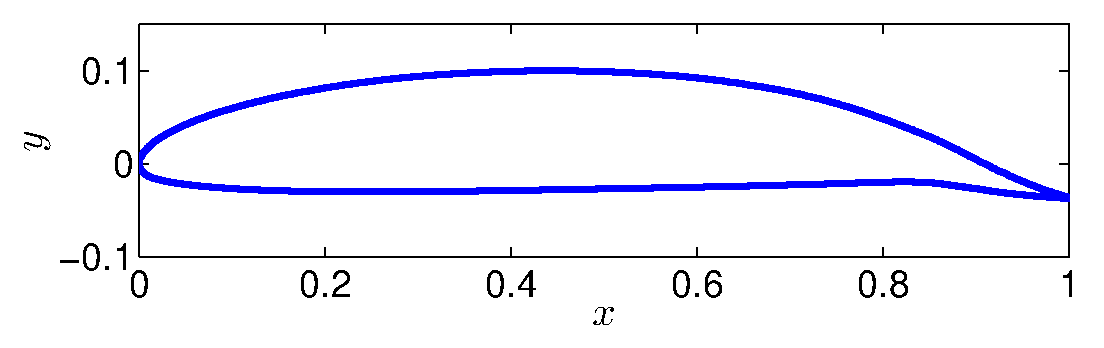
\includegraphics[width=0.9\textwidth]{foil}
	\caption{Natural Laminar Flow (NLF) airfoil extensively tested at the Aeronautical and Vehicle engineering department of KTH \citep{lokatt17,lokattthesis}}
	\label{fig:foil_david}
\end{figure}
Such cases qualitatively represent small changes in operating conditions, such as structural deformations or small trailing edge flap deflections. The understanding of flow response to such changes can be crucial in cases where small perturbations induce large changes in aerodynamic forces. Natural laminar flow (NLF) airfoils may display such sensitive dependence of aerodynamic characteristics for a certain range of angle of attack \emph{viz.} the operating conditions. Their performance critically depends on maintaining laminar flow over the suction side of the airfoil and a loss of laminar flow over the airfoil causes large variations of the aerodynamic forces. Recently \cite{mai11}, and \cite{hebler13} have performed unsteady experiments on natural laminar flows in the transonic range and have found non-linearities in the dynamic response of the normal force coefficients. \cite{lokattthesis} have performed similar experiments within the subsonic range and found strongly non-linear behavior of the normal force coefficient. The non-linearities have been strongly linked to the free movement of transition over the suction side of the airfoil and they appear to be nearly absent when suction side transition is fixed at the leading-edge \citep{mai11,lokattthesis}.

The current work investigates the effect of small-amplitude pitch oscillations on one such laminar airfoil (figure~\ref{fig:foil_david}). The airfoil was designed at the Aeronautical and Vehicle Engineering department of KTH where it has been used in some experimental and numerical works \citep{lokatt17} and is the same airfoil used in the unsteady experiments of \cite{lokattthesis}. The simulations were performed at a chord-based Reynolds number of $Re_{c}=100,000$ within the $\alpha$ range where the above mentioned sensitivity of aerodynamic characteristics to small changes in angle of attack is observed. The sensitive $\alpha$ range for this Reynolds number was determined with calculations using an integral boundary layer code, Xfoil, \cite{drela89}, which predicted sharp changes in the coefficient of moment ($C_{m}$) and suction side transition location (figure~\ref{fig:xfoil_cm}) above an angle of attack $\alpha>6^{\circ}$.
\begin{figure}[h]
	\centering
	\includegraphics[width=0.75\textwidth]{cm-tr-xfoil}
	\caption{Coefficient of moment ($C_{m}$), displayed on the left axis, and suction side transition location, shown on the right axis. Values obtained using Xfoil.}
	\label{fig:xfoil_cm}
\end{figure}

In recent works, wall-resolved large-eddy simulations have proven to be an effective tool for studying flow physics at high Reynolds numbers but with a computational cost which is much lower than that of direct numerical simulations (DNS). Some of the works to utilize this method include spatially evolving boundary layers \citep{eitel14}, pipe flows \citep{chin15} and flow over wings \citep{uzun10,lombard15}. Successful application of the approach has motivated its use in the present work which aims to gain insight into the flow-physics of unsteady airfoils undergoing small amplitude pitch oscillations.
\begin{figure}
	\begin{subfigure}[t]{0.48\textwidth}
		\centering
		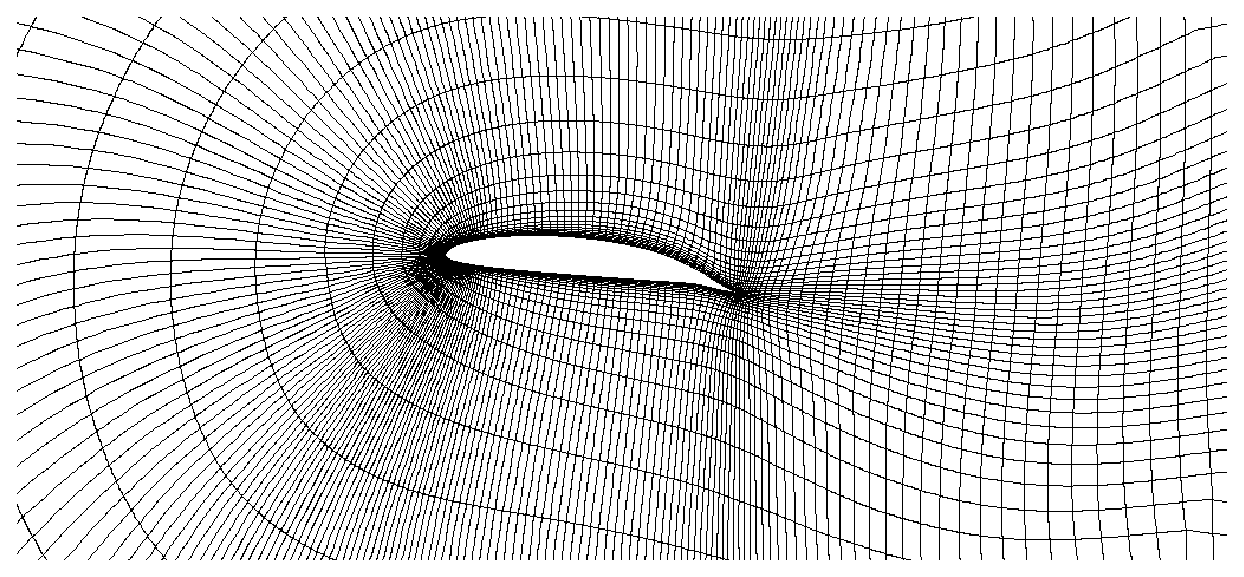
\includegraphics[width=1.\textwidth]{re100k_grid}
		\caption{Spectral element grid.}
		\label{fig:re100k_grid}
	\end{subfigure}
	\begin{subfigure}[t]{0.48\textwidth}
		\centering
		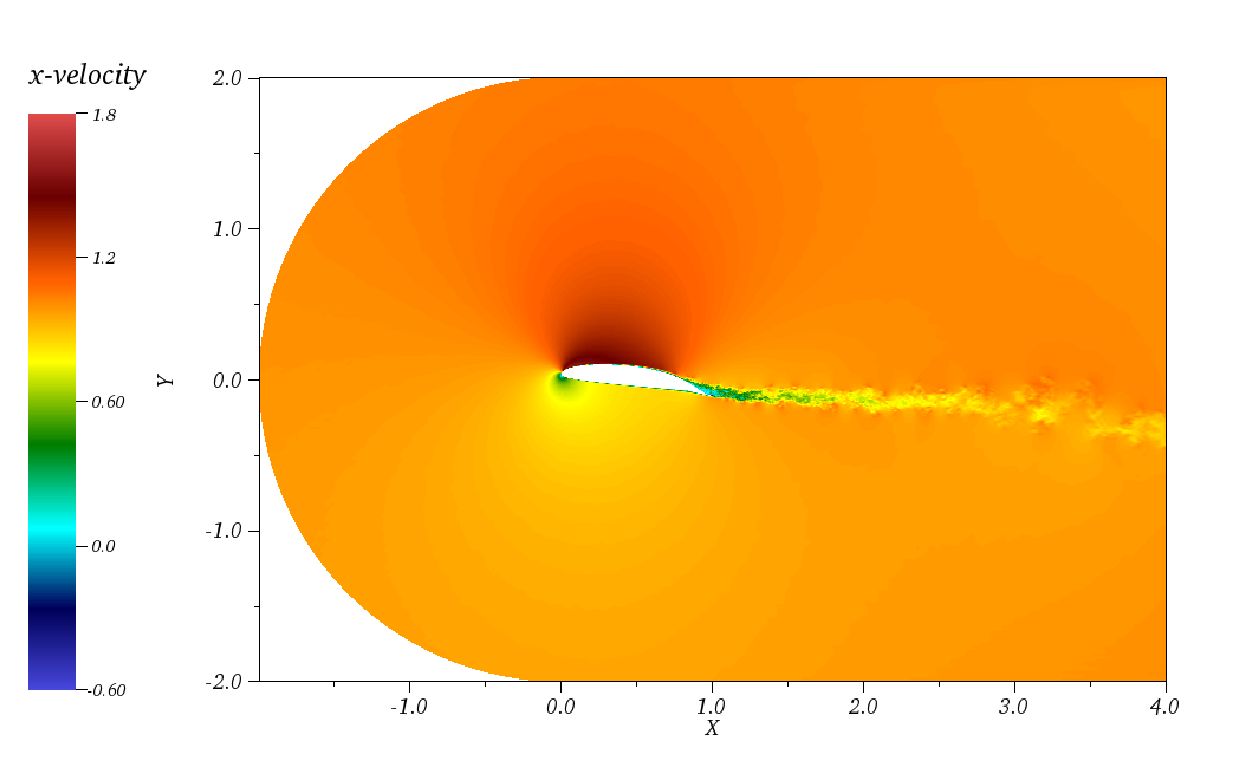
\includegraphics[width=1.0\textwidth]{re100k_grid2}
		\caption{Simulation Domain}
		\label{fig:re100k_domain}
	\end{subfigure}
	\caption{(a) A close-up of the spectral element grid near the airfoil surface. (b) 2D section of the simulation domain: Outflow boundary is $4$ chords downstream of the airfoil leading edge while the inflow boundary is $2$ chords away. Colored region represents the instantaneous streamwise velocity. }	
\end{figure}

\section{Numerical Method}

The computational code used for the simulations is Nek5000, which is an open source research code developed by \cite{nek5000} at Argonne National Laboratory. It is a based on a spectral-element method which allows the mapping of elements to complex geometries along with a high order spatial discretization within the elements. The method uses Lagrange interpolants of orthogonal Legendre polynomials as basis functions and utilizes Gauss--Lobatto--Legendre (GLL) quadrature for the distribution of points within the elements. The spatial discretization is done by means of the Galerkin approximation, following the $P_{N}-P_{N-2}$ formulation. An $11^{th}$ order polynomial approximation is used for the velocity with a $9^{th}$ order approximation for pressure. The nonlinear terms are treated explicitly by third-order extrapolation (EXT3), whereas the viscous terms are treated implicitly by a third-order backward differentiation scheme (BDF3). Aliasing errors are removed with the use of over-integration. All equations are solved in non-dimensional units with the velocities normalized by the reference free-stream velocity $U_{0}$ and the length scales in all directions are normalized by the chord length $c$. The resultant non-dimensional time unit is given by $c/U_{0}$.
%%%%%%%%%%%%%%%%%%%%%%%%%%%%%%%%%%%%%%%%%%%%%%%%%%%%%%%%%%%%%%%%%%%%%%
\subsection{Relaxation-term large-eddy simulation (RT-LES)}

The LES method is based on the RT3D variant of the ADM-RT approach first used by \cite{schlatter04}. The method supplements the governing equations with a dissipative term ($\chi\mathcal{H}(u)$). The equations of motion for the resolved velocity and pressure thus read:
\begin{eqnarray}
\frac{\partial u}{\partial t} + u\cdot\nabla u =  - \frac{1}{\rho}\nabla p + \frac{1}{Re}\nabla^{2}u -\chi\mathcal{H}(u) \\
\nabla\cdot u = 0
\end{eqnarray}
where $\mathcal{H}$ is a defined high-pass spectral filter and $\chi$ is a model parameter which together with $\mathcal{H}$ determines the strength of the dissipative term. The method has been used in earlier studies of boundary layer simulations in \cite{eitel14} and channel flows in \cite{schlatter06}, and has been shown to be reliable in predicting transition location and also preserving the characteristic structures which are seen in the DNS of transitional flows by \cite{schlatter06}.

\subsection{Computational Setup}
A number of tests were carried out in a channel flow at a friction Reynolds number of $Re_{\tau}=395$, and the results are compared with the DNS data of \cite{moser99}. Finally the chosen resolution was set to $\Delta x^{+}=18$, $\Delta z^{+}=9$, with the first point in the wall-normal direction set at $\Delta y_{w}^{+}=0.64$ and the wall-normal resolution near the boundary layer edge is set to $y_{max}^{+}=11$. The superscript $^{+}$ indicates normalization in inner units. The resolution is very similar to the one used in \cite{eitel14} where the ADM-RT model is also used to simulate a spatially evolving boundary layer. A comparison of the results for the turbulent channel flow is shown for the mean velocity in figure~\ref{fig:vel_mean}, and for the turbulent kinetic energy budget (TKE) in figure~\ref{fig:budget}. The dissipation profile shown in the figure is the sum of resolved dissipation and the added dissipation by the relaxation term. A very good agreement with the DNS is found for the mean velocity and all the kinetic energy budget terms (including the total dissipation).

\begin{figure}[h]
	\begin{subfigure}[t]{0.5\textwidth}
		\centering
		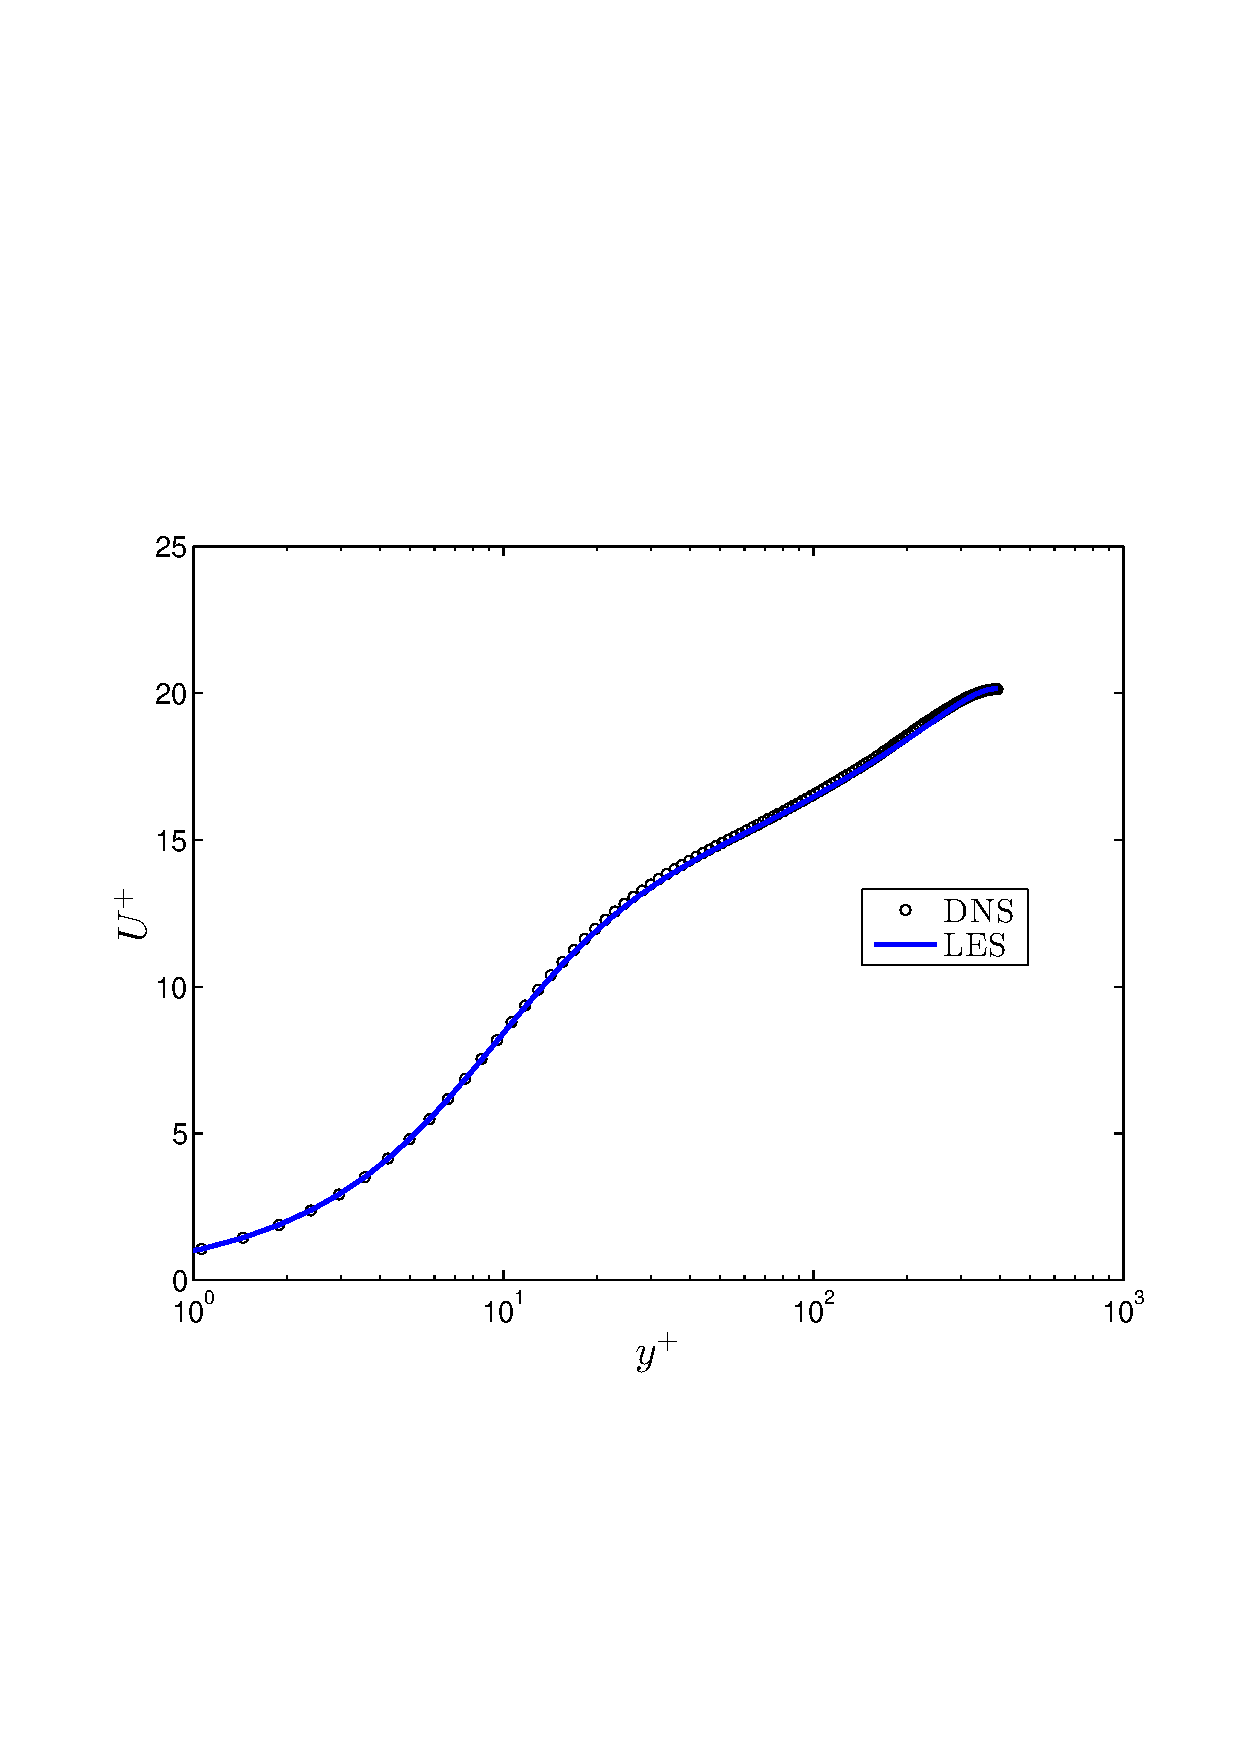
\includegraphics[width=0.95\textwidth]{vel-log}
		\caption{Mean velocity profile.}
		\label{fig:vel_mean}
	\end{subfigure}	
	\begin{subfigure}[t]{0.5\textwidth}
		\centering
		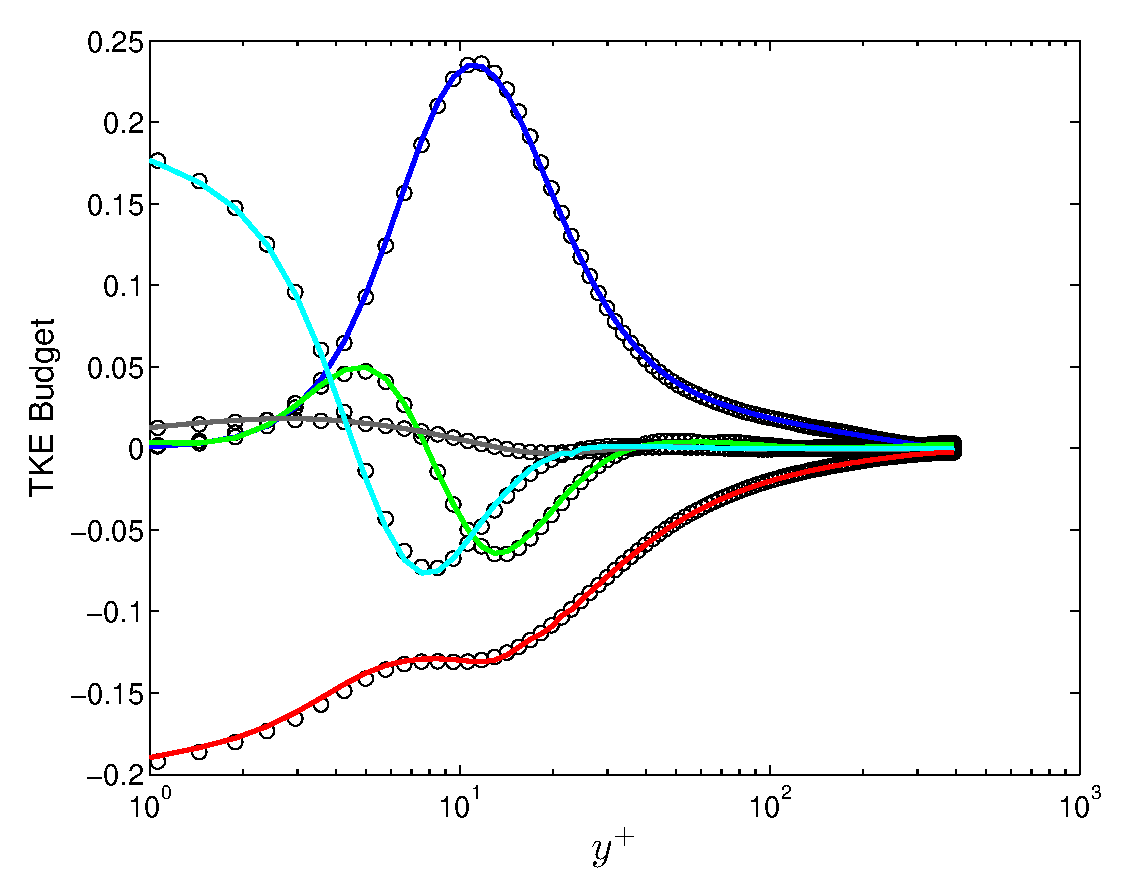
\includegraphics[width=0.98\textwidth]{budgets}
		\caption{Turbulent kinetic energy budget}
		\label{fig:budget}
	\end{subfigure}
	\caption{Comparison of mean velocity profile and turbulent kinetic energy budget. Circles represent the DNS data from \cite{moser99} while the lines represent the values from the LES. All values are normalized with inner units. The individual terms for the turbulent kinetic energy budget in (b) are color coded as: \textcolor{blue}{Production}, \textcolor{red}{Dissipation}, \textcolor{cyan}{Viscous diffusion}, \textcolor{green}{Turbulent diffusion}, \textcolor{mygray}{Velocity-Pressure correlation}}
\end{figure}

The same resolution (in inner units) is then used to design the mesh around the airfoil, with additional care taken for special regions like the leading and trailing edge. Wall-shear stress data is obtained using Xfoil to estimate the grid spacing on the airfoil. A trip is introduced in Xfoil at $x/c\approx0.1$ to obtain turbulent wall-shear values on both the suction and pressure sides of the airfoil. Here $c$ denotes the chord length. Finally, the grid design uses the following criteria:

\begin{itemize}
	\item[$\bullet$] For $0.1<x/c<0.6$, $\Delta x^{+}=18$, $\Delta y_{wall}^{+}=0.64$ and $\Delta y_{max}^{+}=11$, using the local wall-shear ($\tau_{w}$) values on the airfoil. Since the flow is expected to be laminar on the pressure side, the stream-wise resolution is slightly relaxed to $\Delta x^{+}=25$ while keeping the same wall-normal resolution.
	\item[$\bullet$] For $x/c<0.1$, the peak $\tau_{w}$ value over the suction side of the airfoil is used to estimate the grid spacing.
	\item [$\bullet$] for $x/c>0.6$, the suction side experiences a large adverse pressure gradient which significantly reduces $\tau_{w}$ values. Therefore, the $\tau_{w}$ values from the pressure side are used for both the suction and pressure sides.
	\item [$\bullet$] A structured mesh is used, which is extruded in the span-wise direction. Hence the spanwise resolution is constant throughout the domain. The resolution is set to $\Delta z^{+}=9$, where the the peak $\tau_{w}$ value from the suction side is used.
\end{itemize}

A different criterion is needed for defining the resolution in the wake where the wall-based criteria are not valid. Accordingly, RANS simulations were performed using \textit{ANSYS}\textsuperscript{\textregistered} FLUENT, Academic Research, Release 16.1, to estimate the Kolmogorov length scale ($\eta$) in the wake region. The grid in the wake region is designed such that the average grid spacing between the GLL points follows the criteria: $\Delta x/\eta < 9$. The far field boundaries are $2$ chords away from the airfoil leading edge in either direction and the outflow boundary is $4$ chords downstream from the airfoil leading edge. The inlet is designed as a curved inflow boundary with a constant radial distance of $2$ chords from the leading edge of the airfoil. The computational domain is $0.25$ chords wide in the spanwise direction. The domain can be visualized in figure~\ref{fig:re100k_domain}. The spectral-elements can be visualized in the close-up view (figure~\ref{fig:re100k_grid}). Each of the spectral-elements are further discretized by $12\times12\times12$ grid points in 3D, corresponding to an $11^{th}$ order spectral discretization. Periodic boundary conditions are imposed on the spanwise boundaries, while the energy-stabilized outflow condition suggested by \cite{dong2014} is imposed on the outflow boundary. This outflow condition was shown to be accurate and stable in flows with strong back-flow velocities at the outflow boundary by \cite{dong2014}. Velocity field data is extracted from an unsteady RANS simulation and the time-averaged value is interpolated onto the domain inlet and far-field boundaries. The interpolated data is then imposed as a Dirichlet boundary condition on these boundaries. The method is very similar to the one used by \cite{hosseini16} in their DNS of flow around a wing section. In order to simulate low turbulence flight conditions, free-stream turbulence of intensity $Ti=0.1\%$ is superimposed on the Dirichlet boundary conditions. The free-stream turbulence is generated using Fourier modes with a von K\'arm\'an spectrum. The procedure is similar to the one described in \cite{brandt04} and has been used for the study of transition in flat plate boundary layers under the influence of free-stream turbulence.

A validation of the above criterion for complex geometries such as a wing section was performed at a chord based Reynolds number of $Re_{c}=400,000$ for NACA4412 airfoil. The LES grid resolution was setup with the same grid criteria as described above. The domain boundaries and boundary conditions are identical to the setup in \cite{hosseini16}. The results are validated using the DNS data from \cite{hosseini16}. Wall-normal profiles of the normalized kinetic energy budget is shown in figure~\ref{fig:wing_budget}. The profiles are extracted a streamwise location of $x/c=0.7$ on the suction side of the airfoil. The LES profiles (lines) match very well with the DNS data (circles), signifying the high accuracy of the LES with the current resolution.
\begin{figure}[h]
	\centering
	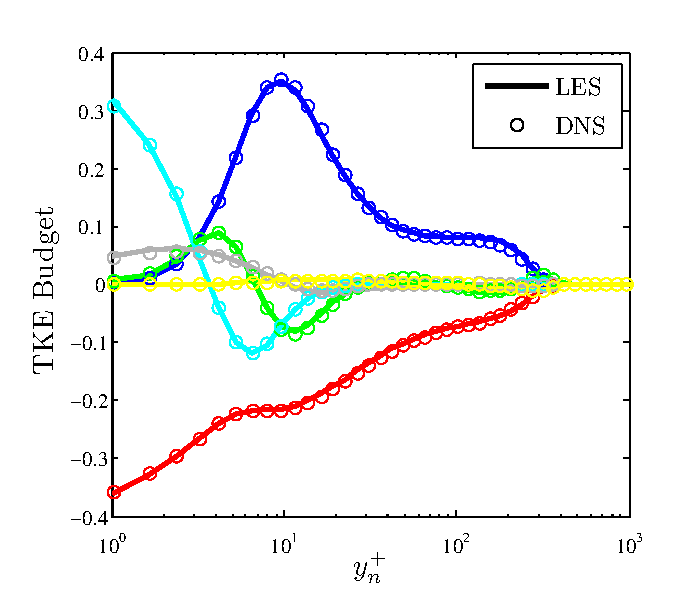
\includegraphics[width=0.6\textwidth]{tke_vs_yp.pdf}
	\caption{Comparison of turbulent kinetic energy budget for a NACA4412 wing section at the suction side location of $x/c=0.7$. The circles represent DNS data from \cite{hosseini16} while the lines are data from the LES. The individual terms are color coded as: \textcolor{blue}{Production}, \textcolor{red}{Dissipation}, \textcolor{cyan}{Viscous diffusion}, \textcolor{green}{Turbulent diffusion}, \textcolor{mygray}{Velocity-Pressure correlation}, \textcolor{yellow}{Convection}}
	\label{fig:wing_budget}
\end{figure}
\section{Results and discussion}
\subsection{Steady results}
% Aoa 6.7 vs aoa 8.0
\begin{figure}[t]
	\begin{subfigure}[b]{0.49\textwidth}
		\centering
		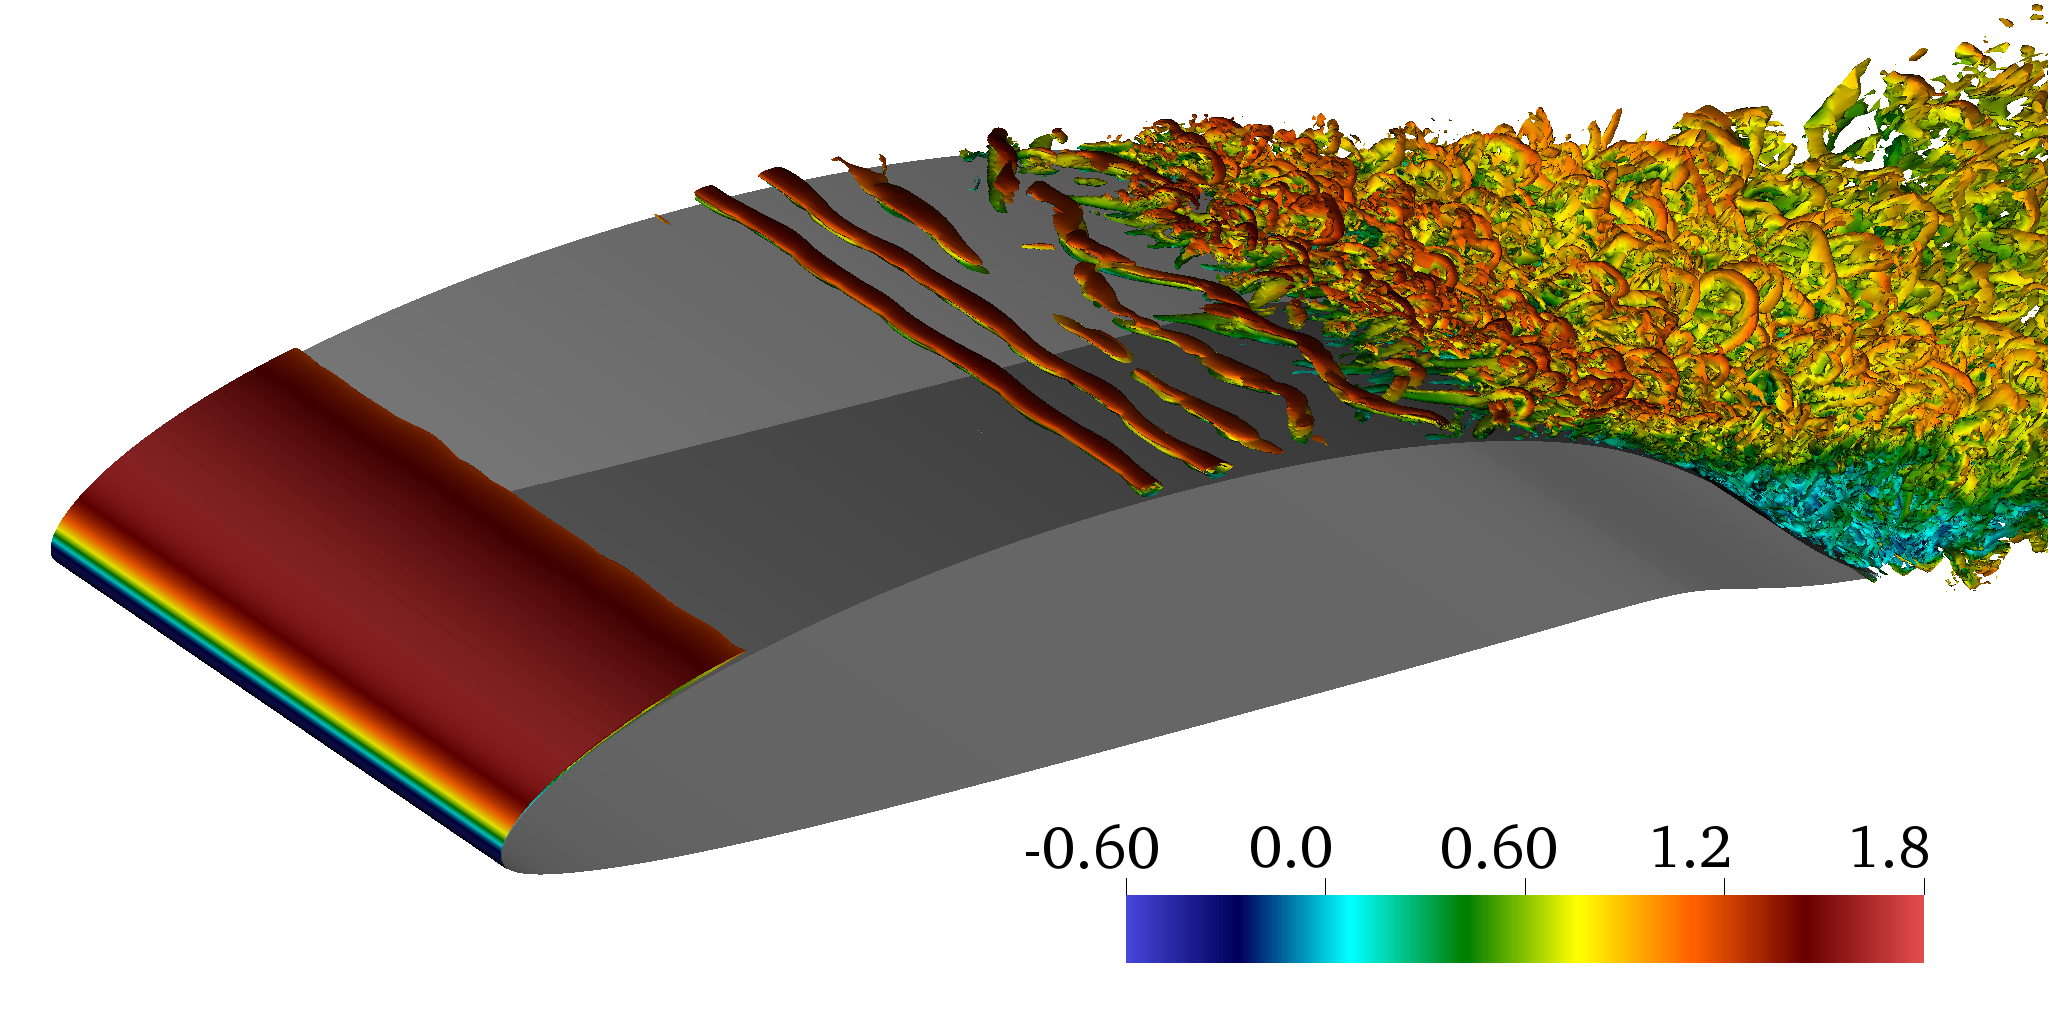
\includegraphics[width=1\textwidth]{re100k_static67_0001}
		\caption{$\alpha=6.7^{\circ}$}
		\label{fig:aoa67_iso}
	\end{subfigure}
	\begin{subfigure}[b]{0.49\textwidth}
		\centering
		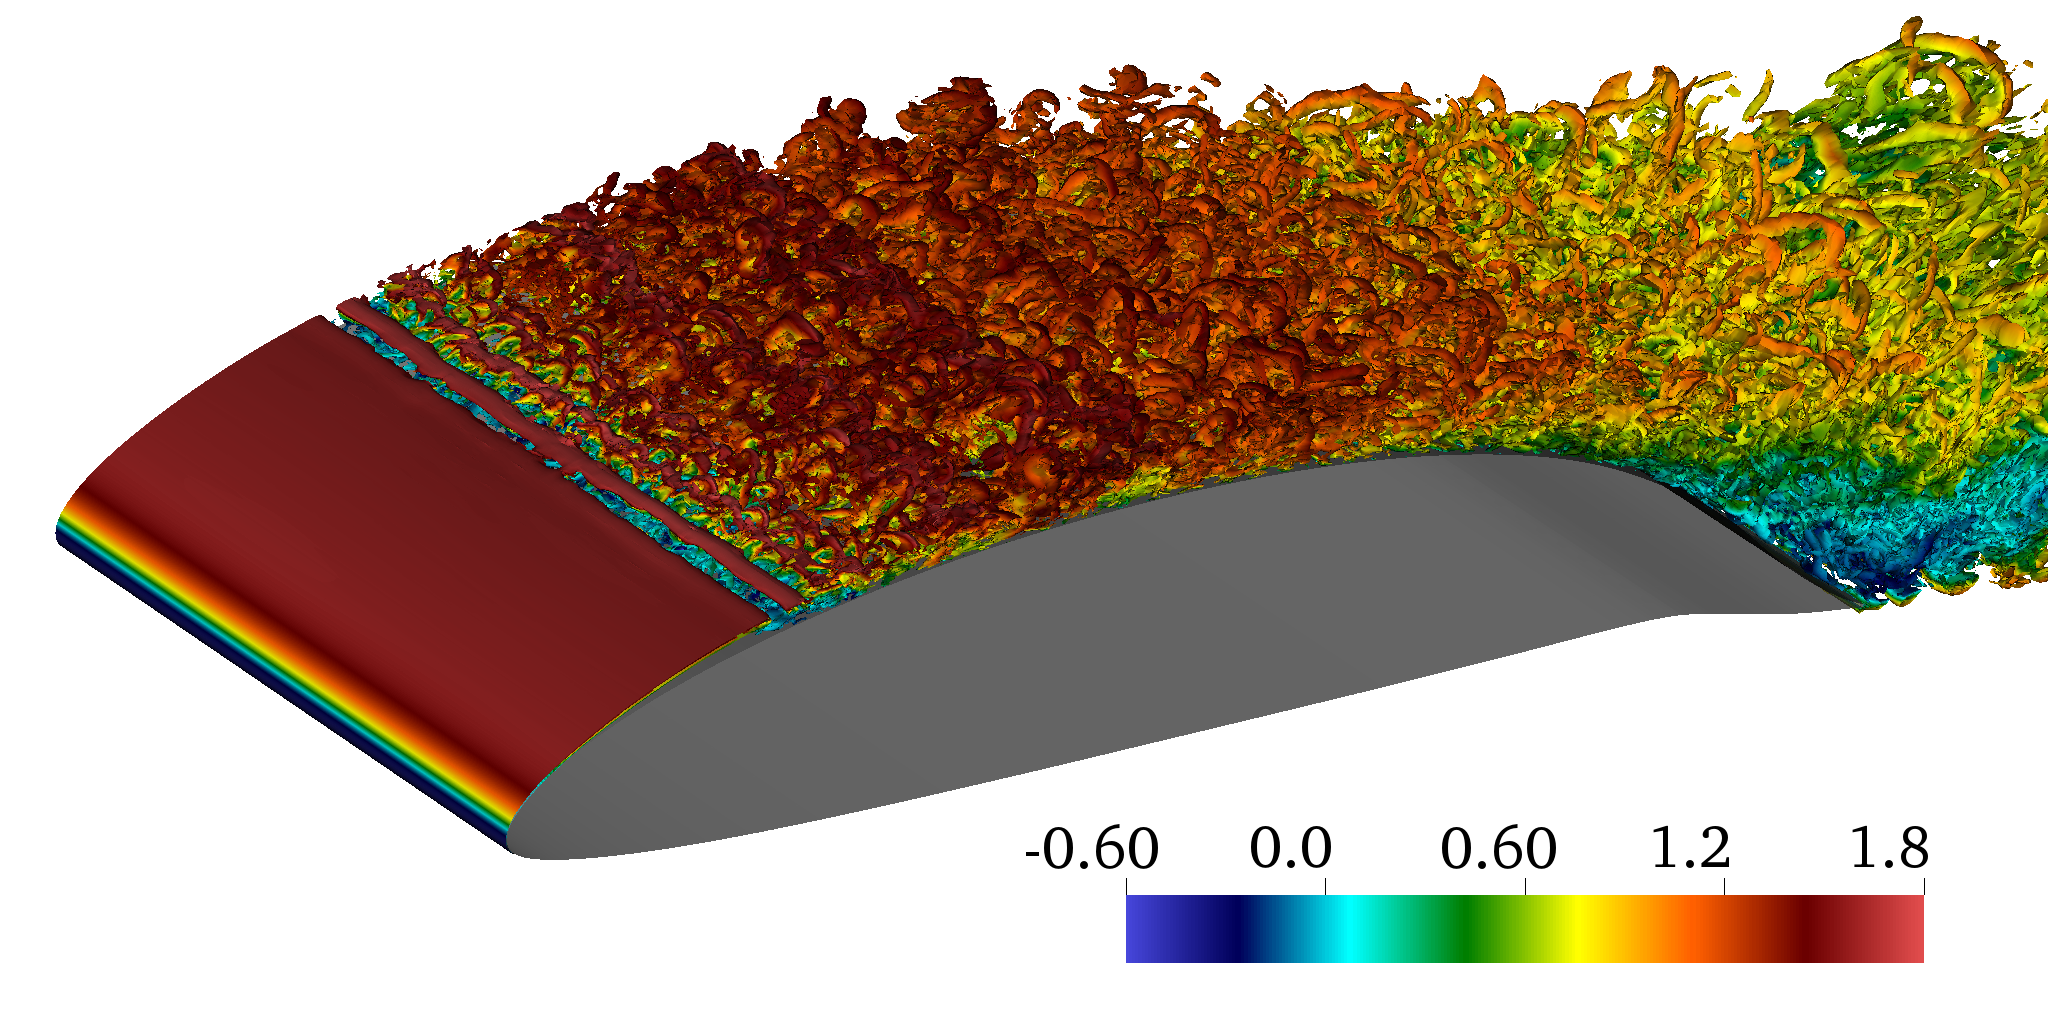
\includegraphics[width=1\textwidth]{re100k_static80_0001}
		\caption{$\alpha=8.0^{\circ}$}
		\label{fig:aoa80_iso}
	\end{subfigure}
	\caption{Isocontours of instantaneous $\lambda_{2}$ structures observed for two different (stationary) angles of attack.}
	\label{fig:isocontour_aoa}
\end{figure}

Simulations with a stationary airfoil were performed to investigate the location of transition without pitching motion. The simulations were performed for $Re_{c}=100,000$ at two different angles of attack ($\alpha=6.7^{\circ}$ and $\alpha=8.0^{\circ}$). As observed in figure~\ref{fig:isocontour_aoa}, the iso-contours of coherent structures, identified by negative $\lambda_{2}$ \citep{jeong95}, show a substantial change in transition location for a small $\Delta\alpha=1.3^{\circ}$. For $\alpha=6.7^{\circ}$ the transition is close to the trailing edge at $x/c\approx0.7$, where due to the effects of strong pressure gradient a small laminar separation bubble develops near $x/c\approx0.6$ and the flow transition occurs at $x/c\approx0.7$. While for $\alpha=8.0^{\circ}$, a leading-edge laminar separation bubble forms, causing flow transition much closer to the leading edge at $x/c\approx0.2$. Such a leading-edge laminar separation bubble is not observed for the $\alpha=6.7^{\circ}$ case. The results are consistent with the trends obtained from Xfoil calculations, showing a large variation in the transition point within a small $\alpha$ change (figure~\ref{fig:xfoil_cm}).
%%%%%%%%%%%%%%%%%%%%%%%%%%%%%%%%%%%%%%%%%%%%%%%%%%%%%%%%%%%%%%%%%%%%%%
\subsection{Pitching results}

Once the transition change is established in the steady simulations, the airfoil is then pitched about a mean $\alpha_{0}=6.7^{\circ}$ with a pitching amplitude of $\Delta\alpha=1.3^{\circ}$ and a reduced frequency of $k=0.5$ about a pitch axis of $(x_{0},y_{0})=(0.35,0.034)$. Where, $k=\frac{\omega c}{2U_{0}}$ with $\omega$ being the angular frequency of oscillation. The motion of the airfoil is prescribed by equation~\ref{eqn:alpha_rule}. The pitching motion corresponds to an oscillation time period of $T_{osc}=2\pi$.
\begin{equation}
\alpha = \alpha_{0} + \Delta\alpha\sin(\omega t)
\label{eqn:alpha_rule}
\end{equation}
The time variation of the coefficient of lift ($C_{L}$) is shown in figure~\ref{fig:cl-time-alpha} where the blue line shows the $C_{L}$ values and the dashed black line shows the variation of $\alpha$ with time. The initial phase of pitching motion is carried out using a lower resolution (polynomial order $N=5$) to simulate the initial transient period of the flow at a lower computational cost. The polynomial order is then smoothly raised to $N=11$ before the fourth pitch cycle. Due to the fairly large separation at the trailing edge, effects of transition movement and turbulence, successive pitch cycles are not expected to have identical behavior, however some of qualitatively repeating trends can be observed. The behavior of the lift coefficient shows a chaotic but qualitatively repeating pattern where the lift coefficient shows a fairly smooth increase during the pitch-up motion, with strong secondary effects occurring near the maximum of the pitch cycles. Similarly in the pitch-down phase the lift decreases smoothly with secondary effects again becoming important at the minima of the pitch-cycle.
\begin{figure}[h]
%	\begin{subfigure}[t]{0.5\textwidth}
		\centering
		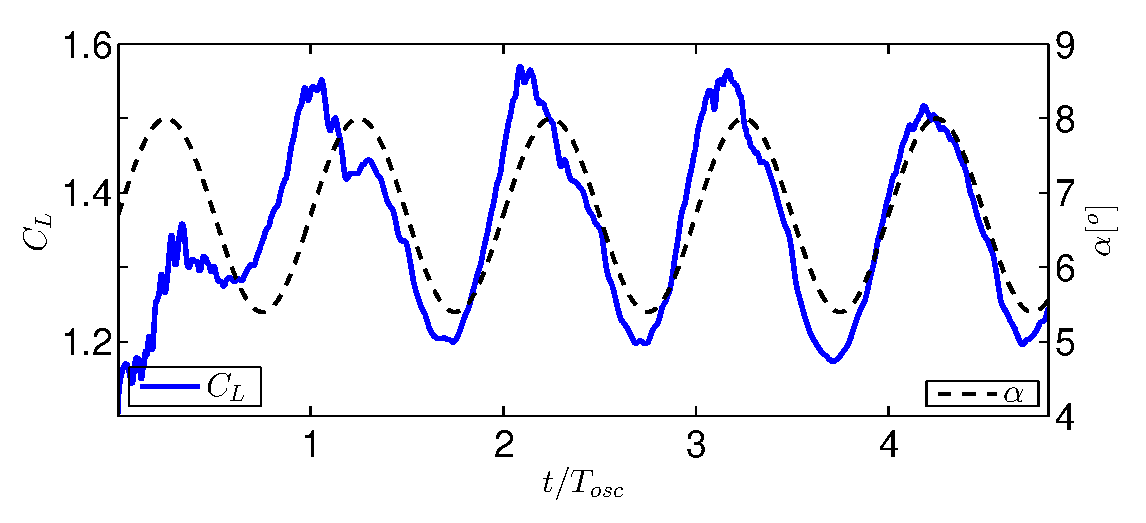
\includegraphics[width=0.9\textwidth,height=0.5\textwidth]{cl-time-alpha}
%		\caption{Time variation}
		\caption{Coefficient of Lift ($C_{L} \textcolor{blue}{-}$) and angle of attack $(\alpha \textcolor{black}{--})$ variation with time. $C_{L}$ is on the left axes while $\alpha$ is on the right axes.}
		\label{fig:cl-time-alpha}
%	\end{subfigure}
%	\begin{subfigure}[t]{0.45\textwidth}
%		\centering
%		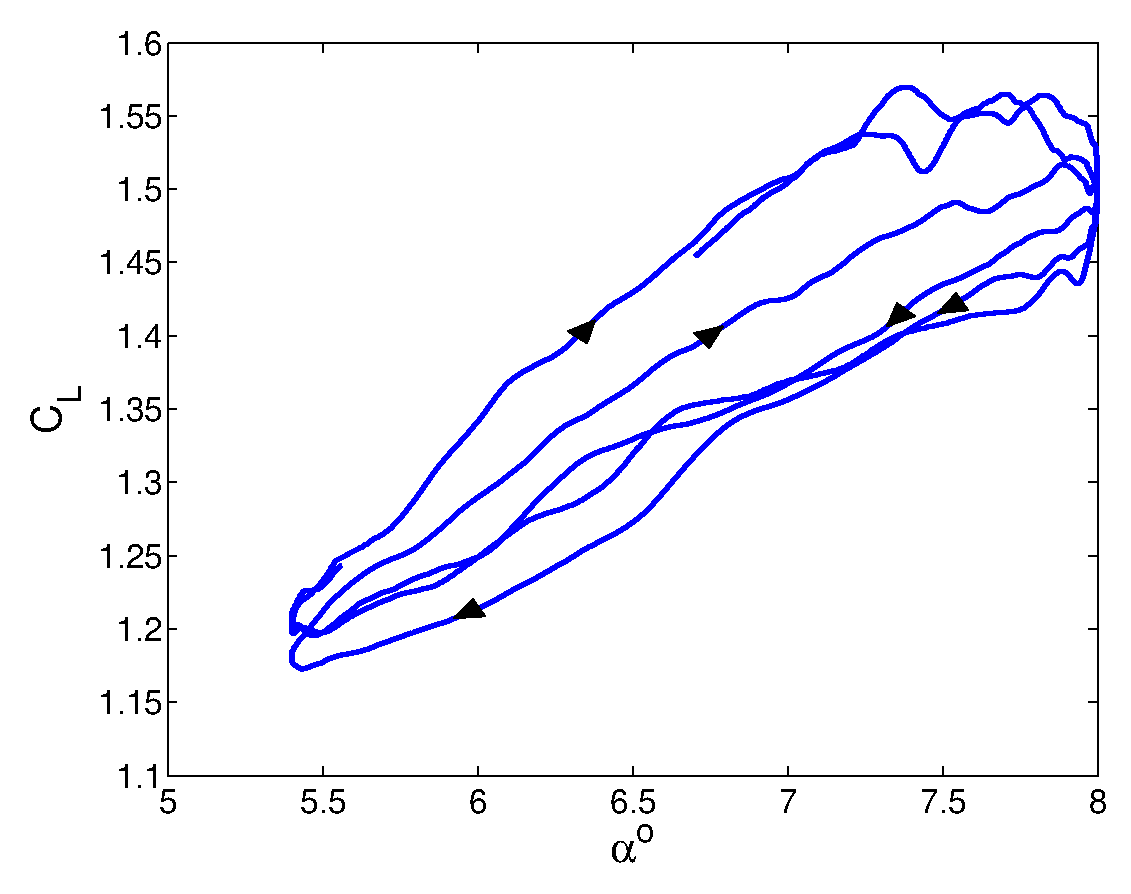
\includegraphics[width=1\textwidth]{cl-alpha}
%		\caption{Phase portrait}
%		\label{fig:cl-alpha}
%	\end{subfigure}
%	\caption{Coefficient of Lift ($C_{L} \textcolor{blue}{-}$) and angle of attack $(\alpha \textcolor{black}{--})$ variation with time (a) . $C_{L}$ is on the left axes while $\alpha$ is on the right axes. Phase portrait of $C_{L}$ and $\alpha$ (b). The sense of motion in figure (b) is clockwise, as marked by the arrows.}
\end{figure}

In order to understand the time variation of the spatially developing boundary layer on the airfoil, we look at the space-time evolution of the instantaneous spanwise averaged wall-shear stress. The space-time surface plot is shown in figure~\ref{fig:cf-time}, which spans the fourth and fifth pitch cycles. The $x-axis$ indicates the chord-wise location on the suction side of the airfoil while the $y-axis$ indicates the simulation time normalized with the time period of oscillation ($T_{osc}$). The color specifies the value of wall-shear stress on the suction side of the airfoil. Regions with color intensity strongly towards red are indicative of high shear and thus turbulent flow. The exception to the rule being the region close to the leading edge where the flow is laminar but a high shear region exists due to the extremely thin boundary layer close to the stagnation point. The same space-time surface is plotted again as a binary colored surface plot in figure~\ref{fig:separation-time}, where black colored regions indicate negative wall-shear stress and hence separated flow, while the white region corresponds to locations with attached flow ($\tau_{w}>0$). Horizontal dashed lines mark specific phases of the pitch cycle. Red dashed line indicates mean instantaneous angle of attack, while blue dashed lines indicate the extreme positions of the instantaneous angle of attack. 
\begin{figure}[h]
	\centering
	\begin{subfigure}[t]{0.46\textwidth}
		\centering
		\includegraphics[width=1\textwidth, height=1.5\textwidth]{cf_time_surf100k}
		\caption{wall-shear stress ($\tau_{w}$).}. 
		\label{fig:cf-time}
	\end{subfigure}
	\begin{subfigure}[t]{0.45\textwidth}
		\centering
		\includegraphics[width=0.97\textwidth, height=1.5\textwidth]{cf_time_surf_grey100k}
		\caption{Separated regions (black).} 
		\label{fig:separation-time}
	\end{subfigure}
	\caption{Space-time plot for the wall-shear values ($\tau_{w}$) and separated flow regions. The values are obtained from the instantaneous flow averaged over the spanwise direction. Horizontal blue dashed lines in \ref{fig:separation-time} represent the extremum positions of angle of attack, while the red dashed lines represent phases corresponding to mean angle of attack.}
	\label{fig:space-time}
\end{figure}

It is obvious from the two plots in figure~\ref{fig:space-time}, that the developing boundary layer on the airfoil exhibits a dynamically rich response to small-amplitude pitch oscillations, with different key boundary layer characteristics controlling the dynamics of the flow in different phases of the pitch cycle. We briefly identify some of the key boundary layer characteristics to paint an over-all picture of the dynamics. A persistent trailing edge separation can be identified in figure~\ref{fig:separation-time} beyond $x/c>0.8$. The trailing-edge separation is does not exhibit reverse flow 100\% of the time, as can be seen from the white patches dispersed between largely black colored regions. An isolated separated region (distinct from the trailing edge separation) is seen at $x/c\approx0.6$ at times $t/T_{osc}\approx3$ and $t/T_{osc}\approx4$. This is identified as a trailing-edge LSB. This LSB is short lived in time, existing for slightly less than a quarter of the pitch-cycle. A large separated region near the leading edge is a leading-edge LSB, similar to the one seen in the steady case at $\alpha=8.0^{\circ}$. The separation bubble persists much longer in time, spanning nearly half a pitch cycle. Thus the flow dynamics may broadly be described as an oscillation between states corresponding to the leading edge and trailing edge laminar separation bubbles. Evident from figure~\ref{fig:cf-time} is that the transition point changes substantially throughout the pitch cycle. Interestingly, the flow over the airfoil is substantially different between the pitch-up and the pitch-down phases for the same angle of attack. For example, when the instantaneous angle of attack is at phase $\phi=0\ (t/T_{osc}=3,\ 4)$, which represents mean angle of attack but in the pitch-up phase, the flow over the airfoil is mostly laminar up till $x/c\approx0.7$. On the other hand, for a phase of $\phi=\pi\ (t/T_{osc}=3.5,\ 4.5)$, representing the airfoil at the mean angle of attack but in the pitch-down phase, the flow is almost entirely turbulent with the start of the turbulent region approximately at $x/c\approx0.25$.

In the current work we focus on the variation of transition location throughout the pitch cycles. Since the flow case is unsteady, and the transition location does not remain fixed, the standard procedure of specifying transition location using flow intermittency is no longer feasible and a different criteria is needed to determine the instantaneous transition location. In order to determine transition, we calculated flow statistics which are averaged in the homogeneous spanwise direction, and also averaged for a short duration ($\Delta t$) in time. Thus the instantaneous value of any statistical quantity ``$\overline{q}(x,y,t)$'' can be evaluated as in equation~\ref{eqn:inst_q}:
\begin{align}
	\overline{q}(x,y,t) = \left(\frac{1}{z_{max}-z_{min}}\right)\left(\frac{1}{\Delta t}\right)\int_{t'=t}^{t'=t+\Delta t}\int_{z=z_{min}}^{z=z_{max}}q(x,y,z,t')\ dz\ dt'
	\label{eqn:inst_q}
\end{align}

In order for such a quantity to be representative of the instantaneous state of the flow, the time duration of the averaging must be small. For the current case we use $\Delta t=4\times10^{-3}$, which amounts to $0.06\%$ of the oscillation time period during which the flow can be assumed to remain in the same state. Using this procedure we evaluate the fluctuating Reynolds stress, $\overline{u'v'}(x,y,t)$, in order to determine the instantaneous transition location. Within the boundary layer region above the suction-side, the location where the absolute value of the quantity first becomes larger than a certain threshold, that point is denoted as the transition point. In order to prescribe a suitable threshold, the maximum value of $|\overline{u'v'}(x,y,t)|$ across the entire boundary layer is evaluated for all times. This maximum value does not have very large variations staying within the same order of magnitude for all times with its mean value being $|\overline{u'v'}|_{max}=0.05$. The threshold for determining transition is set to $5\%$ of this value. The transition point is thus the first point where $|\overline{u'v'}(x,y,t)|>0.0025$. Since we use an ad-hoc criteria for transition location, this is cross-checked by evaluating the variance of the spanwise velocity fluctuations $\overline{w'w'}(x,y,t)$, and following an identical procedure as described above. In this case the transition criteria is prescribed as $|\overline{w'w'}(x,y,t)|>0.005$ since the peak spanwise fluctuation intensities are found to be higher than the peak Reynolds stress $|\overline{u'v'}|$. Physically, growing spanwise velocity fluctuations indicate the onset of three-dimensionality in the boundary layer, which are associated with secondary instabilities. While the thresholds specified may be considered ad-hoc, the qualitative picture of transition movement is not very sensitive to small changes in the threshold. Reducing the thresholds by a factor of 2 still produces the same qualitative trends (not shown). Figure~\ref{fig:space-time_tr} shows the calculated transition locations overlay-ed on the wall-shear stress and separation space-time plots. The calculated transition locations are consistent with the picture of wall-shear stress with transition marginally preceding regions of turbulent flow. Moreover, the time variation of transition point determined by two different physical quantities agree very well with each other. Thus we consider the quantities as a good representation of changing flow characteristics.
\begin{figure}[h]
	\centering
	\begin{subfigure}[t]{0.45\textwidth}
		\centering
		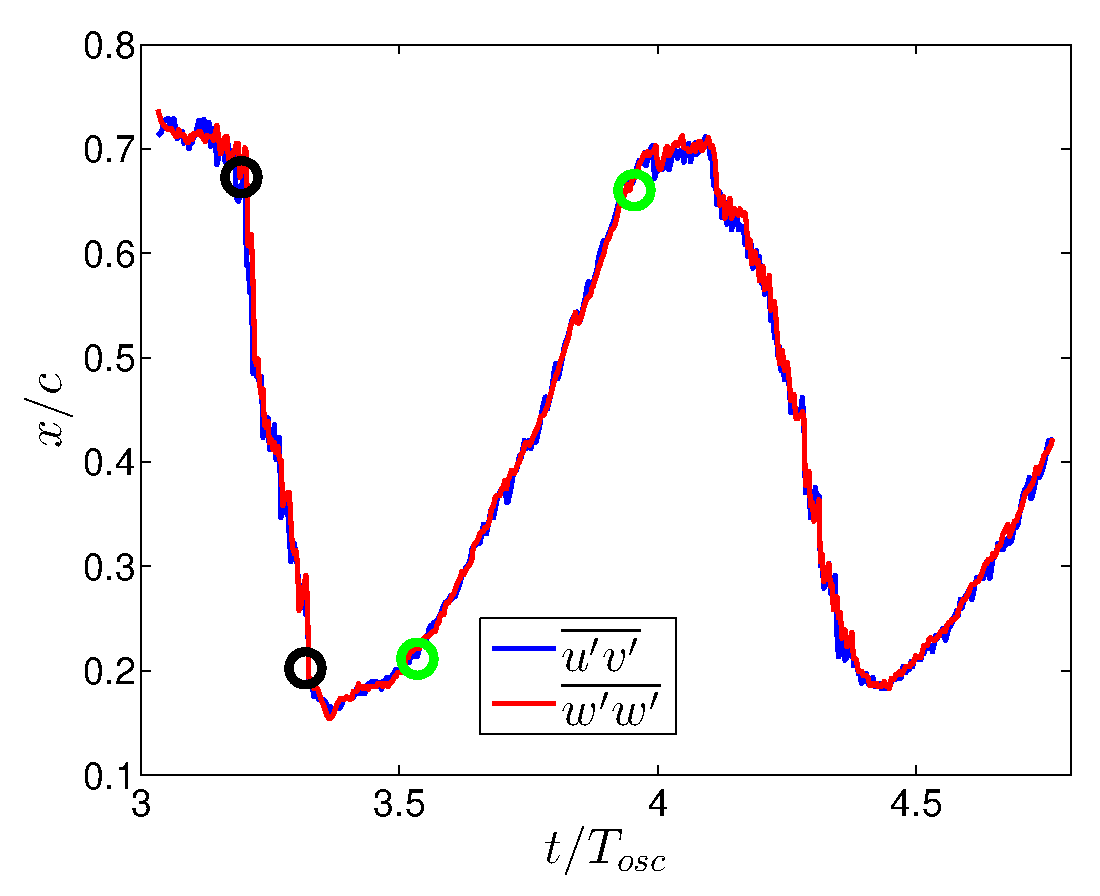
\includegraphics[width=1\textwidth]{transition_time}
		\caption{Transition variation with time.}. 
		\label{fig:transition_time}
	\end{subfigure}
	\begin{subfigure}[t]{0.45\textwidth}
		\centering
		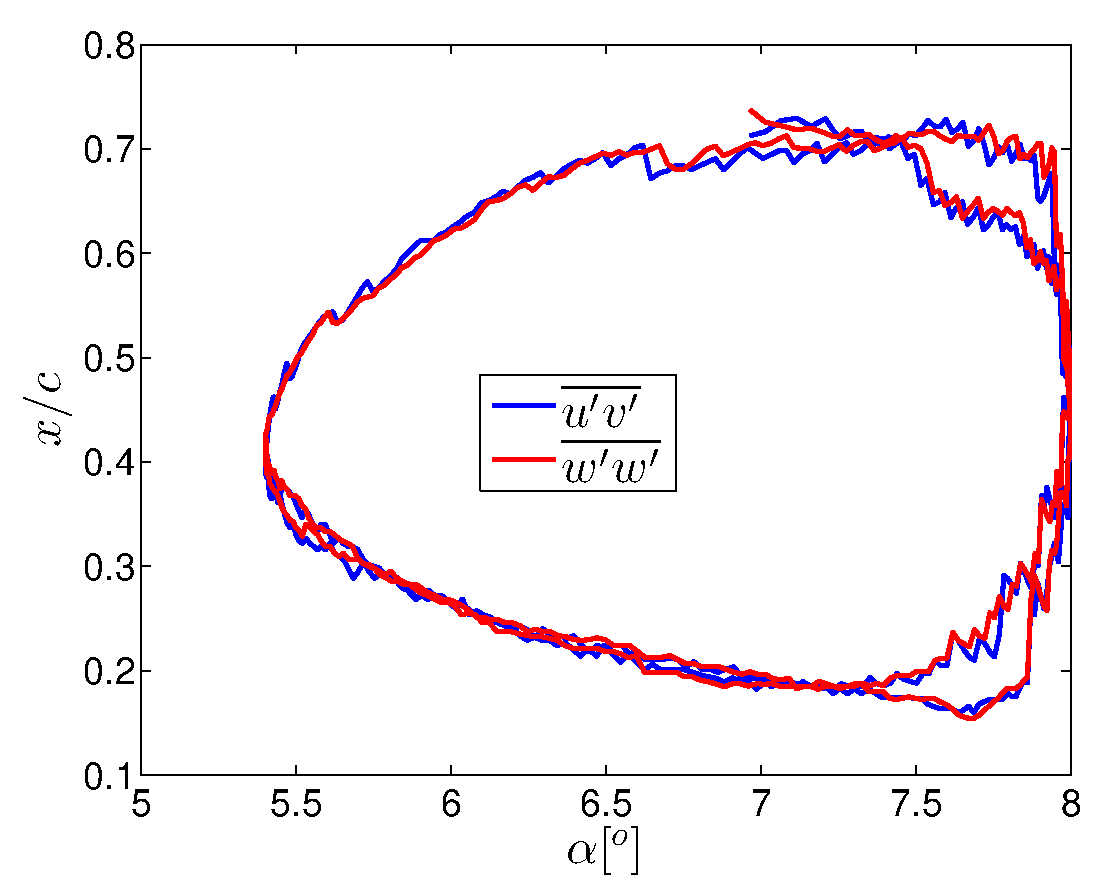
\includegraphics[width=1\textwidth]{transition_alpha}
		\caption{Transition location phase portrait.} 
		\label{fig:transition_alpha}
	\end{subfigure}
	\caption{Time variation (a) and phase portrait with $\alpha$ (b) of transition location evaluated using the criteria for $|u'v'|$ and $|w'w'|$. The circles mark the points used to approximate the upstream (black circles) and downstream (green circles) velocities of the transition point.}
	\label{fig:transition}
\end{figure}

The overlay plots in figure~\ref{fig:space-time_tr} clearly indicate that the two LSBs play a dominating role in the flow dynamics and that transition location is governed by the characteristics of these LSBs. Figure~\ref{fig:transition_la2} shows the instantaneous iso-contours of the $\lambda_{2}$ structures at four different times during the pitch-up cycle when the transition is moving upstream. The top figure shows the flow state near the mean angle of attack ($t/T_{osc}=3.09$) during the pitch-up phase. The flow is mostly laminar across the wing with no structures seen prior to flow transition. The high adverse pressure gradient near the trailing edge causes the laminar flow to easily separate, forming a laminar separation bubble and flow transitions over this separated shear layer. The next figure from the top is at the time instant $t/T_{osc}=3.2$ and the leading edge LSB has formed which excites spatially growing waves as seen by the quasi two-dimensional vortical structures captured by the $\lambda_{2}$ criteria. As the LSB grows in size, the spatially growing waves undergo stronger amplification and transition downstream of the leading-edge LSB (third figure from top at $t/T_{osc}=3.3$). The flow downstream of the point of transition is now turbulent and thus does not separate from the surface. The LSB near the trailing edge therefore ceases to exist. Finally, the leading-edge LSB grows large enough that flow transitions within this separated shear layer (bottom figure at $t/T_{osc}=3.47$). The growth of the leading-edge LSB can be quantified in terms of the maximum reverse flow observed within recirculation region. Figure~\ref{fig:backflow_ratio} shows the absolute value of the maximum reverse flow within the circulation region normalized by the free-stream velocity at the boundary layer edge. \cite{alam00} with their local stability analysis of a two-parameter family of reverse flow profiles indicated that reverse flow intensities above $15\%$ may cause the flow to be locally absolutely unstable. With a similar analysis on a three parameter family of profiles \cite{hammond98} obtained onset of absolute instabilities at $20\%$ reverse flow velocities. The authors also performed global stability analysis on a synthetically created boundary layer with a symmetric separation bubble \citep{hammond98} and found the flow to be globally unstable for $30\%$ reverse flow velocities. In the current flow case reverse flow intensities of up to $40\%$ can be observed shortly before transition occurs within the separated shear layer of the leading edge LSB. This is much higher than the onset of absolute instability reported in the earlier studies and while we do not perform a formal stability analysis in the current study, it is reasonable to assume the leading-edge LSB becomes globally unstable, and causes transition at the separated shear layer. 
\begin{figure}[h]
	\centering
	\begin{subfigure}[t]{0.46\textwidth}
		\centering
		\includegraphics[width=1\textwidth, height=1.5\textwidth]{cf_time_surf100k_tr}
		\caption{Wall-shear stress ($\tau_{w}$).}. 
		\label{fig:cf-time_tr}
	\end{subfigure}
	\begin{subfigure}[t]{0.45\textwidth}
		\centering
		\includegraphics[width=0.97\textwidth, height=1.5\textwidth]{cf_time_surf_grey100k_tr}
		\caption{Separated regions (black).} 
		\label{fig:separation-time_tr}
	\end{subfigure}
	\caption{Transition locations indicated by the magenta line overlayed on the space-time plots of wall-shear stress and separation.}
	\label{fig:space-time_tr}
\end{figure}

During the pitch down phase of the oscillation cycle, the leading-edge LSB shrinks in size and eventually ceases to be globally unstable. The transition point then starts moving downstream from the leading-edge LSB and the flow over the airfoil begins a slow re-laminarization process. There is a marked asymmetry between the upstream and downstream movement of the transition point. An approximate velocity for both the upstream and downstream motion of the transition point is calculated across the points marked by circles in figure~\ref{fig:transition_time} which correspond to transition movement with near constant velocity. The velocity of upstream transition movement is calculated across the black circles and is equal to $V^{tr}_{u}=-0.60$ while the velocity of the downstream motion of transition is calculated across the green circles and is equal to $V^{tr}_{d}=0.17$. Thus the upstream spread of turbulent regions is much faster than the re-laminarization. At the moment it is unclear what causes the asymmetry between the upstream and downstream movement of transition, or if symmetric movement can even be expected. The cause of this asymmetry will be the focus of future work.
\begin{figure}
	\centering
	\begin{subfigure}[t]{0.48\textwidth}
		\centering
		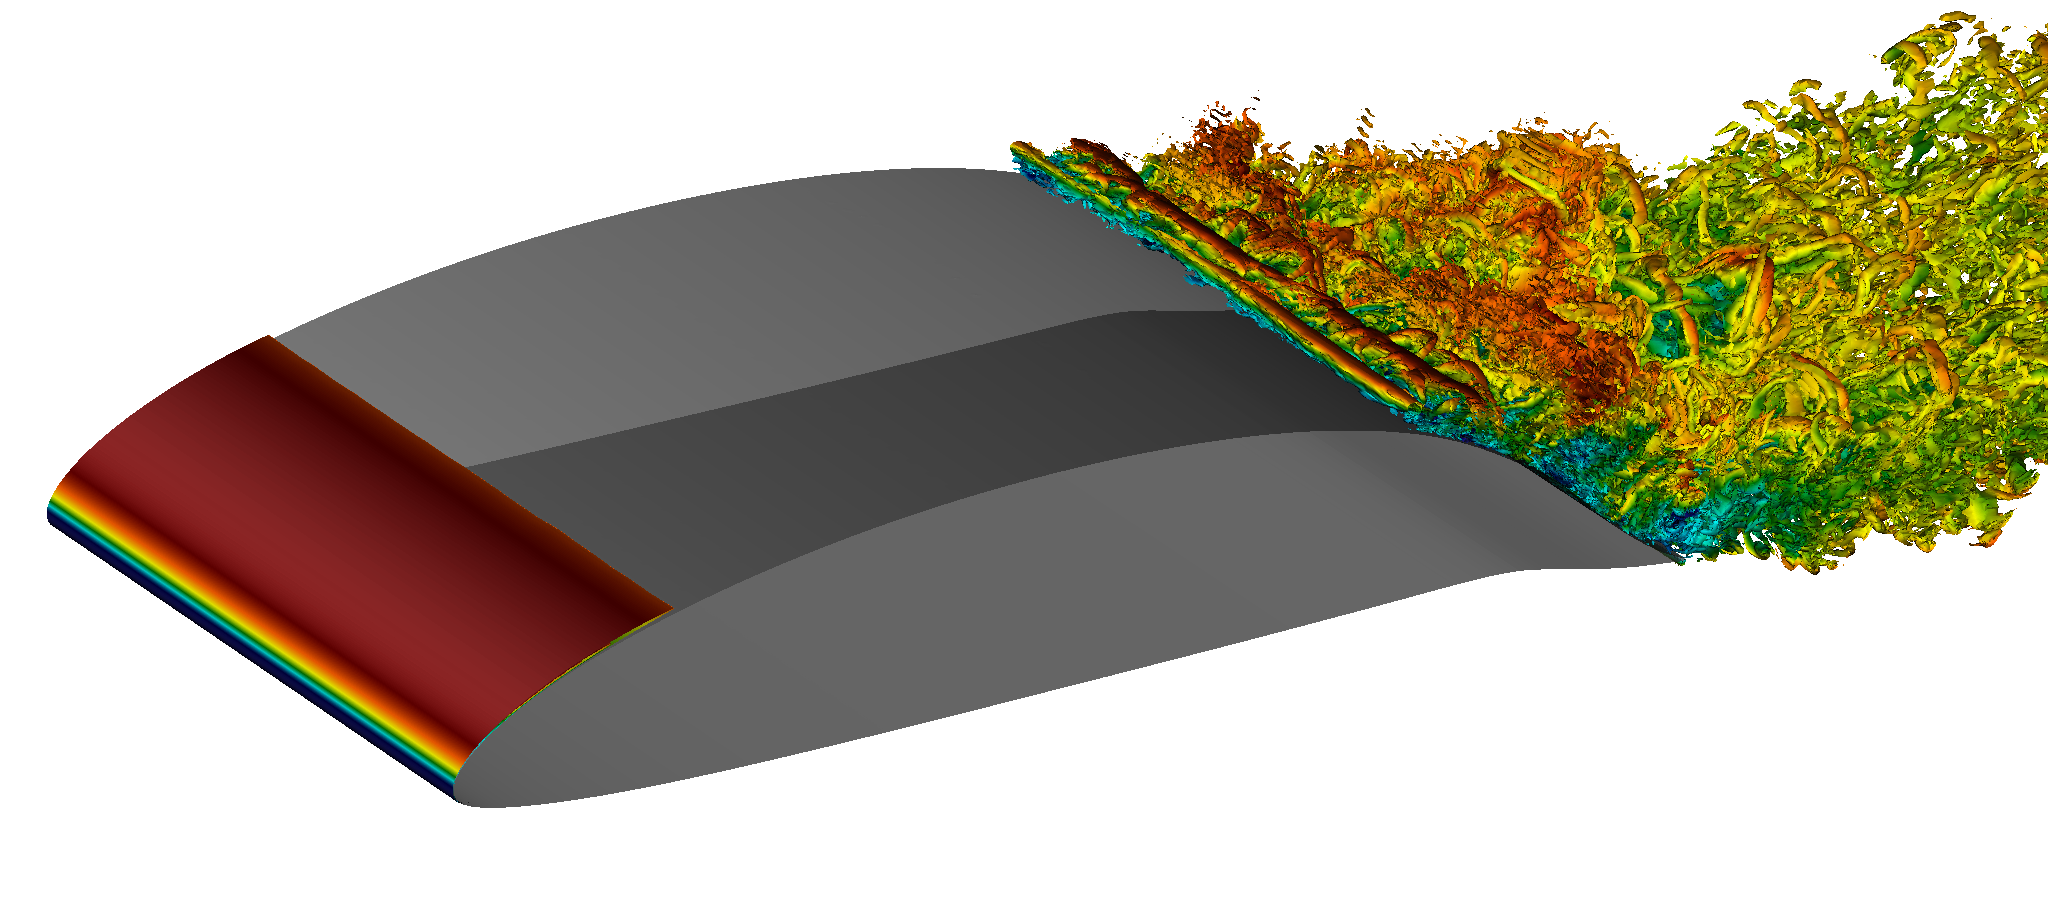
\includegraphics[width=1\textwidth]{pitchup0001.png}
		\label{fig:pitchup_1}
	\end{subfigure}
	\begin{subfigure}[t]{0.48\textwidth}
		\centering
		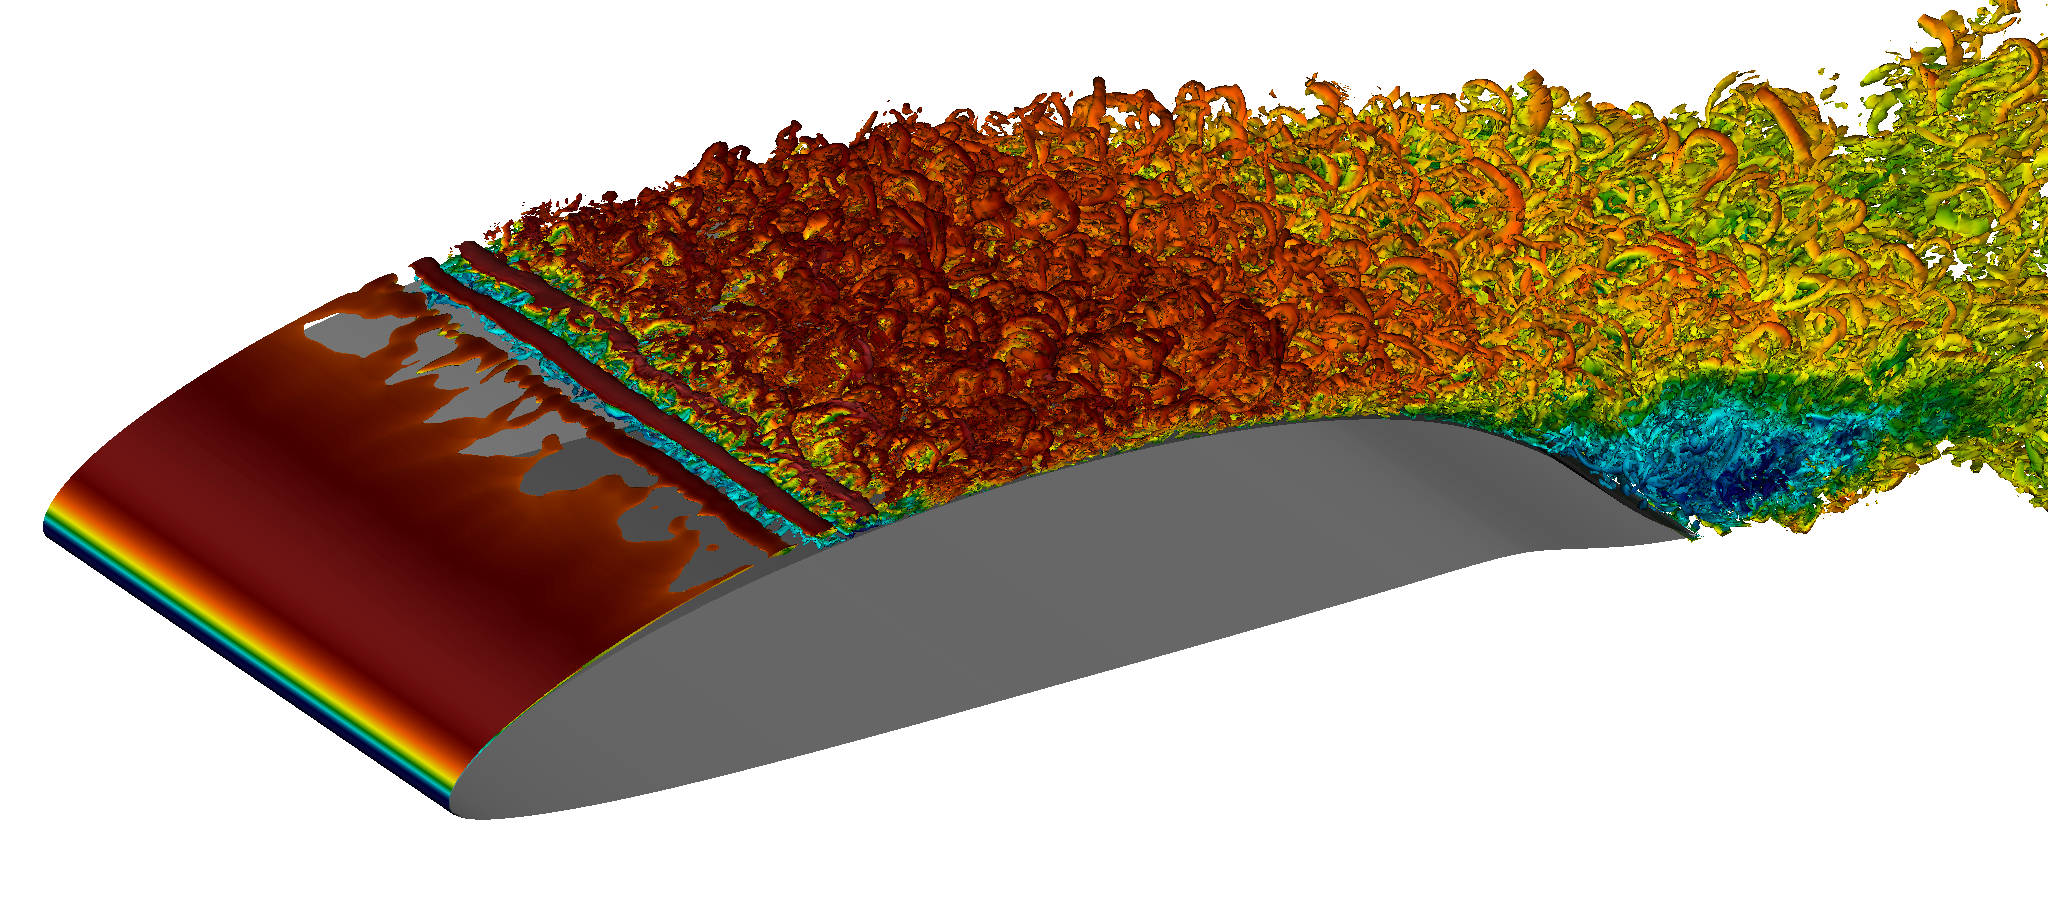
\includegraphics[width=1\textwidth]{relaminar0001.png}
		\label{fig:relaminar_1}
	\end{subfigure}
	\begin{subfigure}[t]{0.49\textwidth}
		\centering
		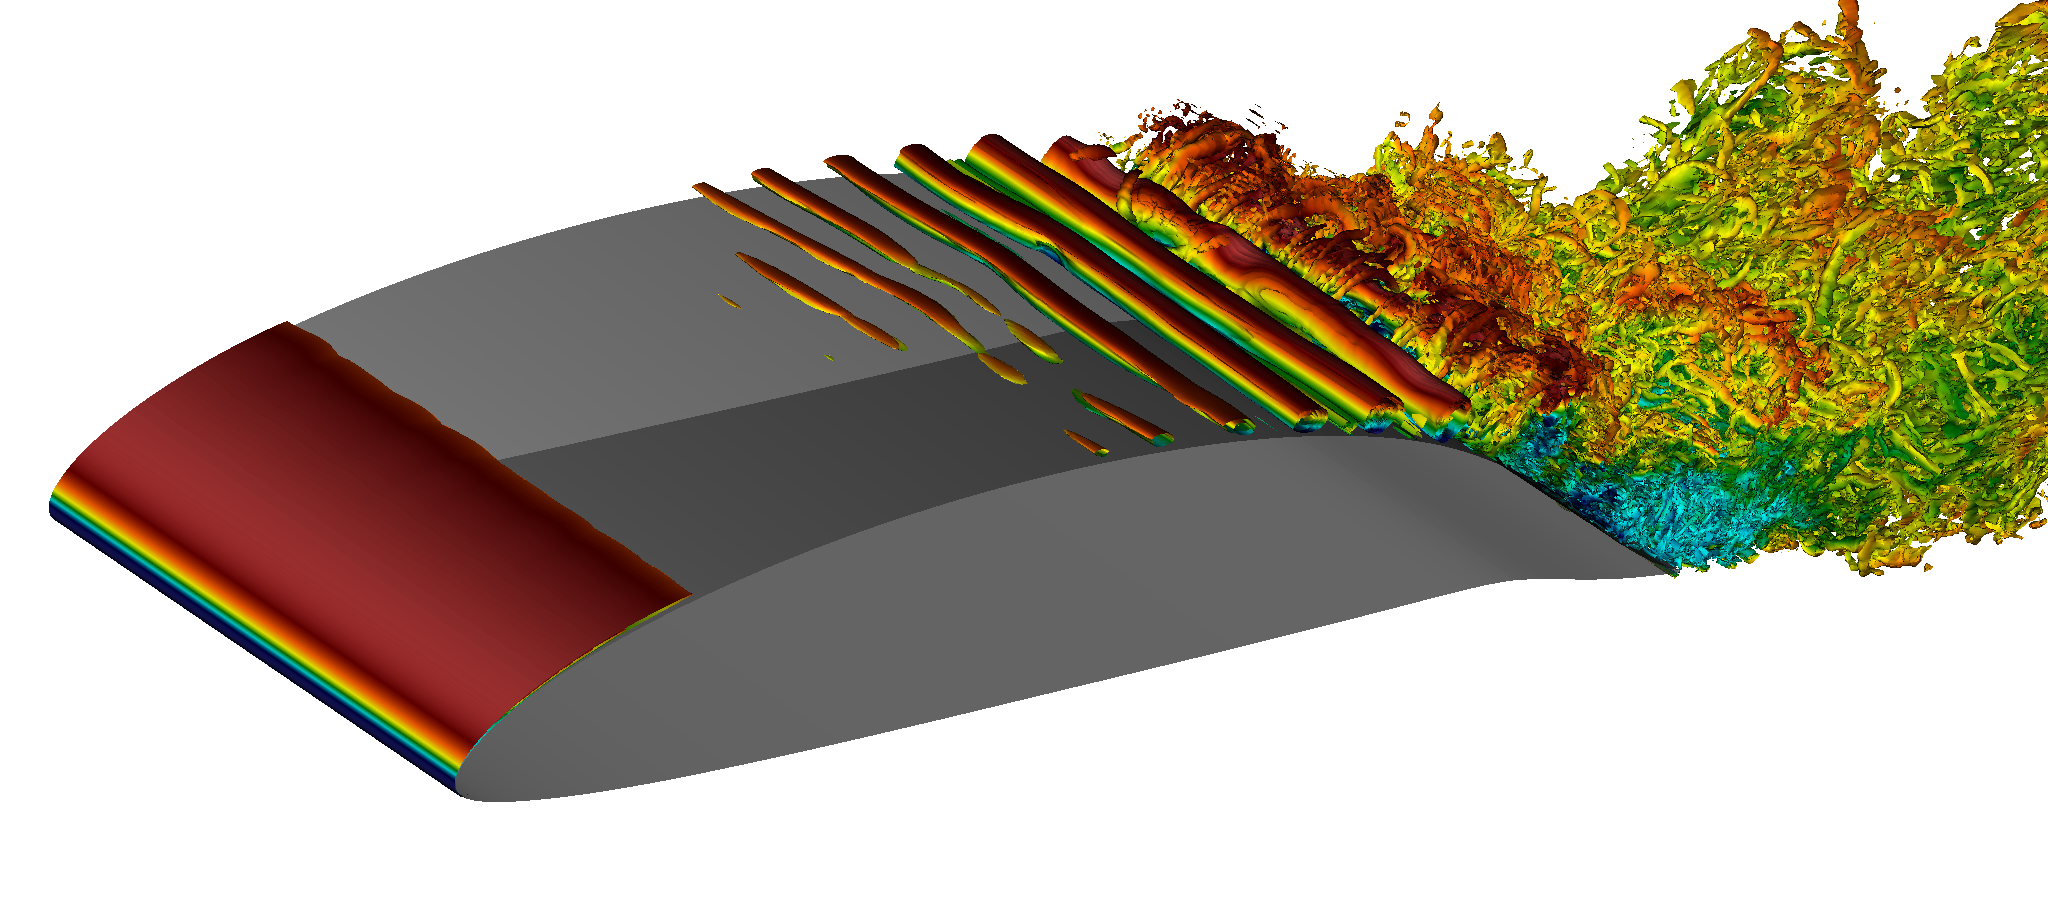
\includegraphics[width=1\textwidth]{pitchup0002.png}
		\label{fig:pitchup_2}
	\end{subfigure}
	\begin{subfigure}[t]{0.49\textwidth}
		\centering
		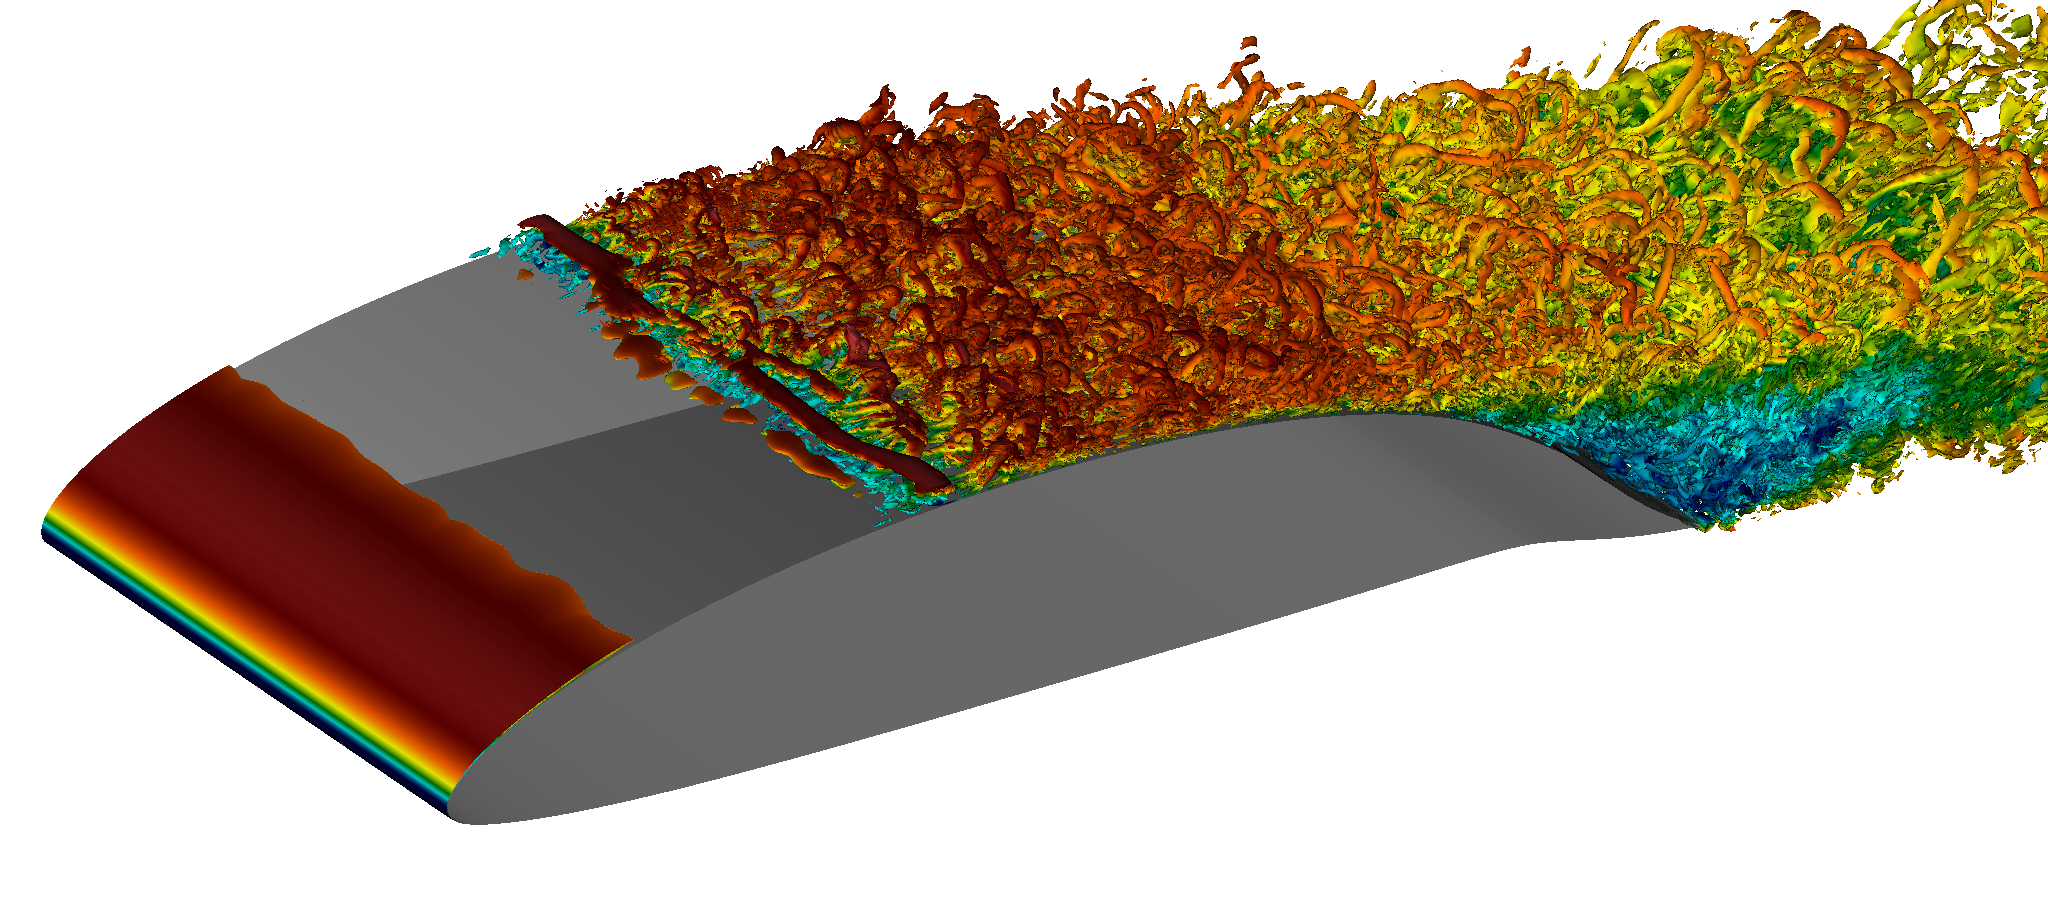
\includegraphics[width=1\textwidth]{relaminar0002.png}
		\label{fig:relaminar_2}
	\end{subfigure}
	\begin{subfigure}[t]{0.49\textwidth}
		\centering
		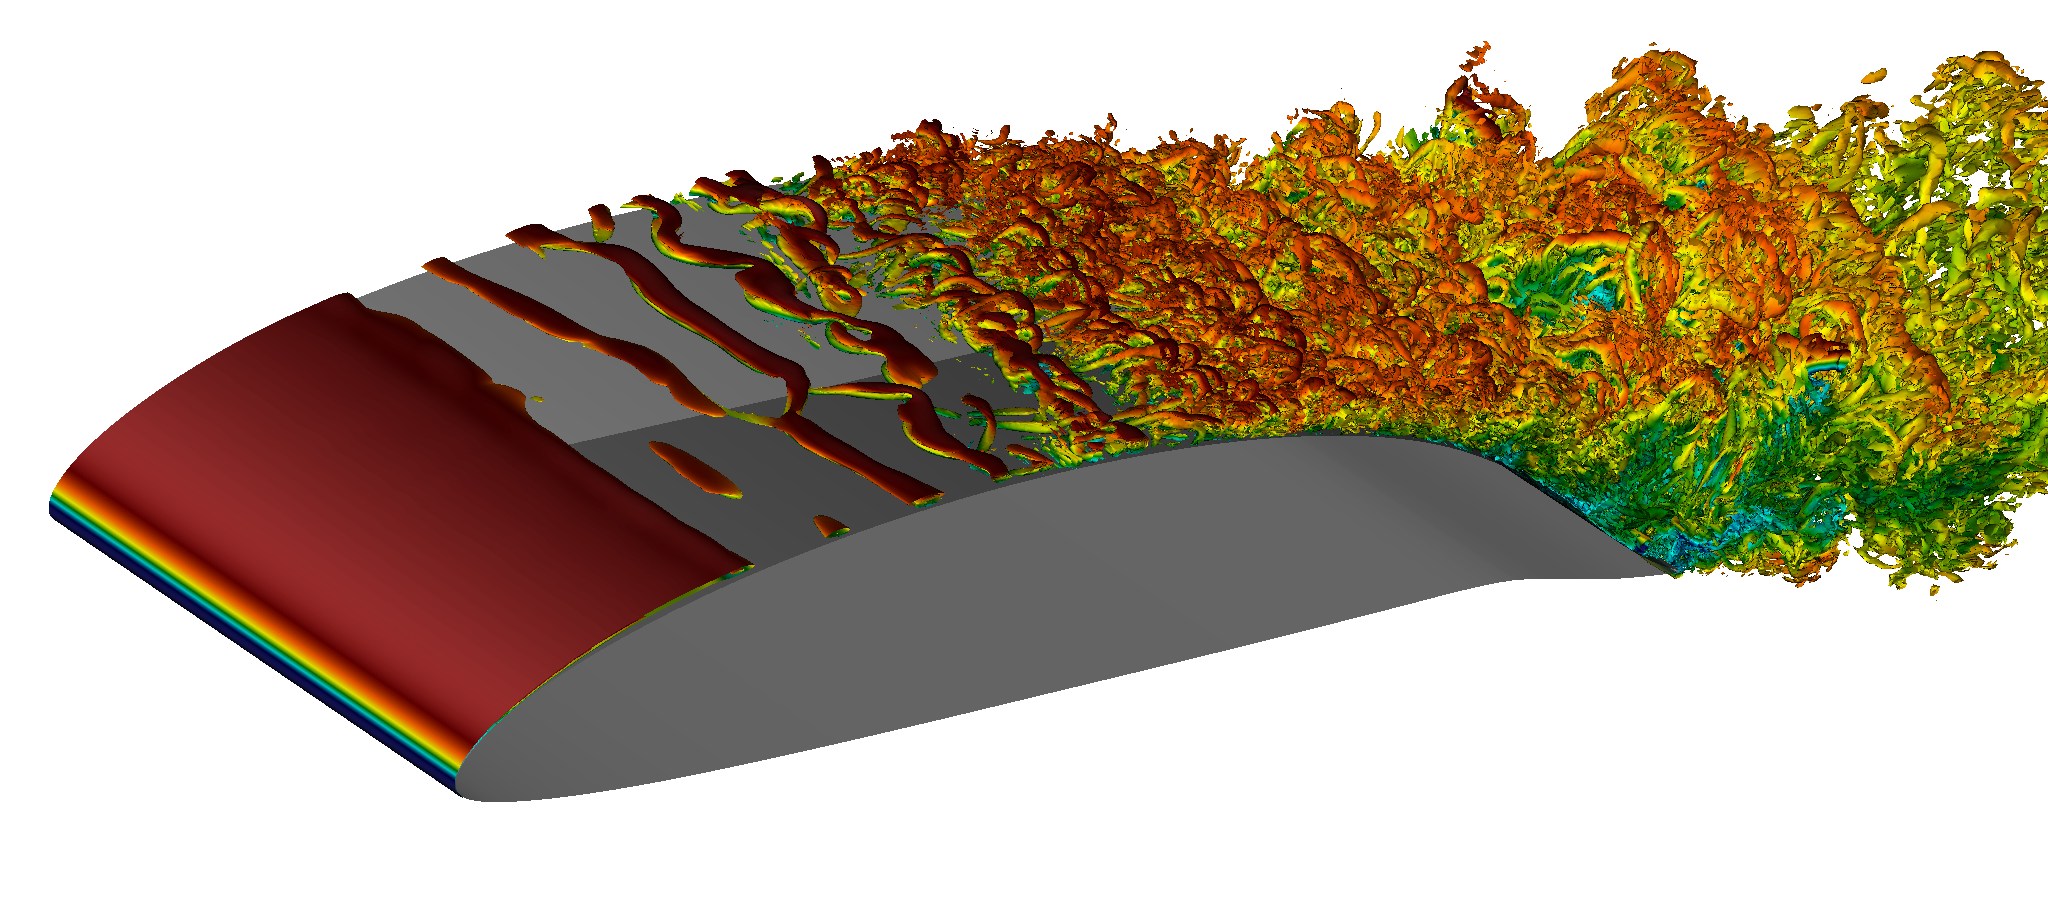
\includegraphics[width=1\textwidth]{pitchup0003.png}
		\label{fig:pitchup_3}
	\end{subfigure}
	\begin{subfigure}[t]{0.49\textwidth}
		\centering
		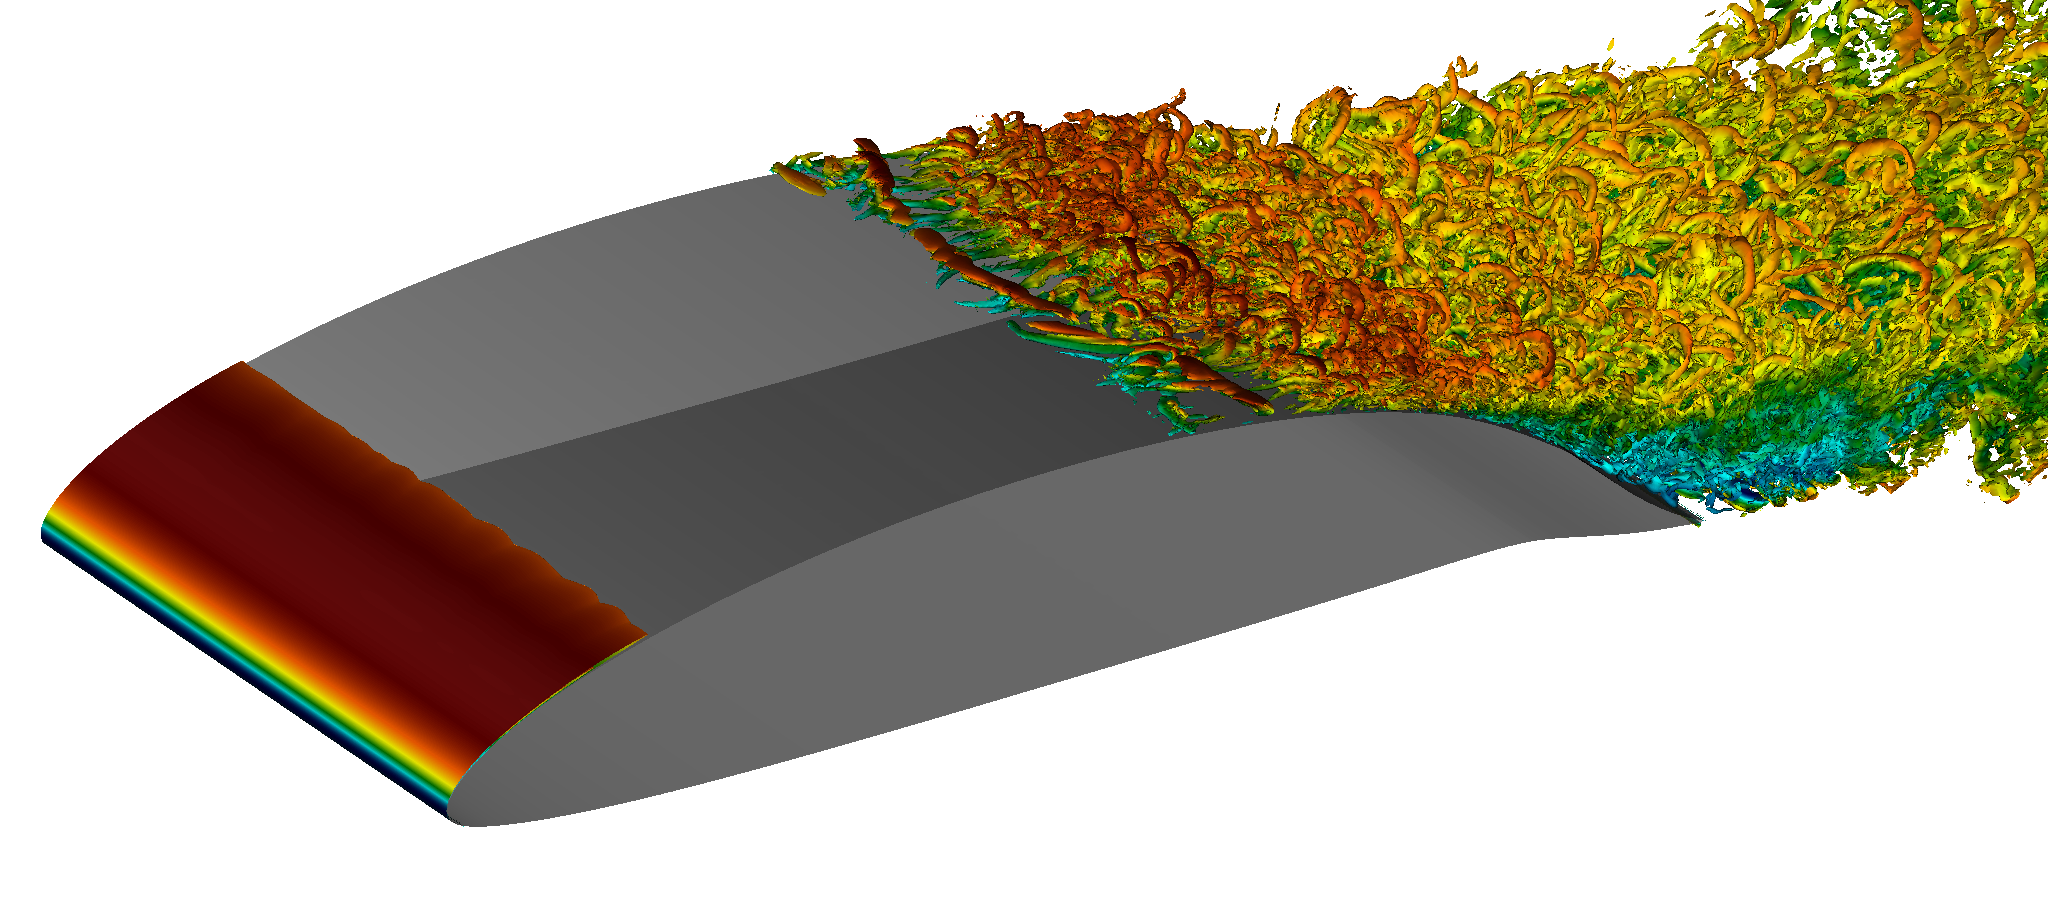
\includegraphics[width=1\textwidth]{relaminar0003.png}
		\label{fig:relaminar_3}
	\end{subfigure}
	\begin{subfigure}[t]{0.49\textwidth}
		\centering
		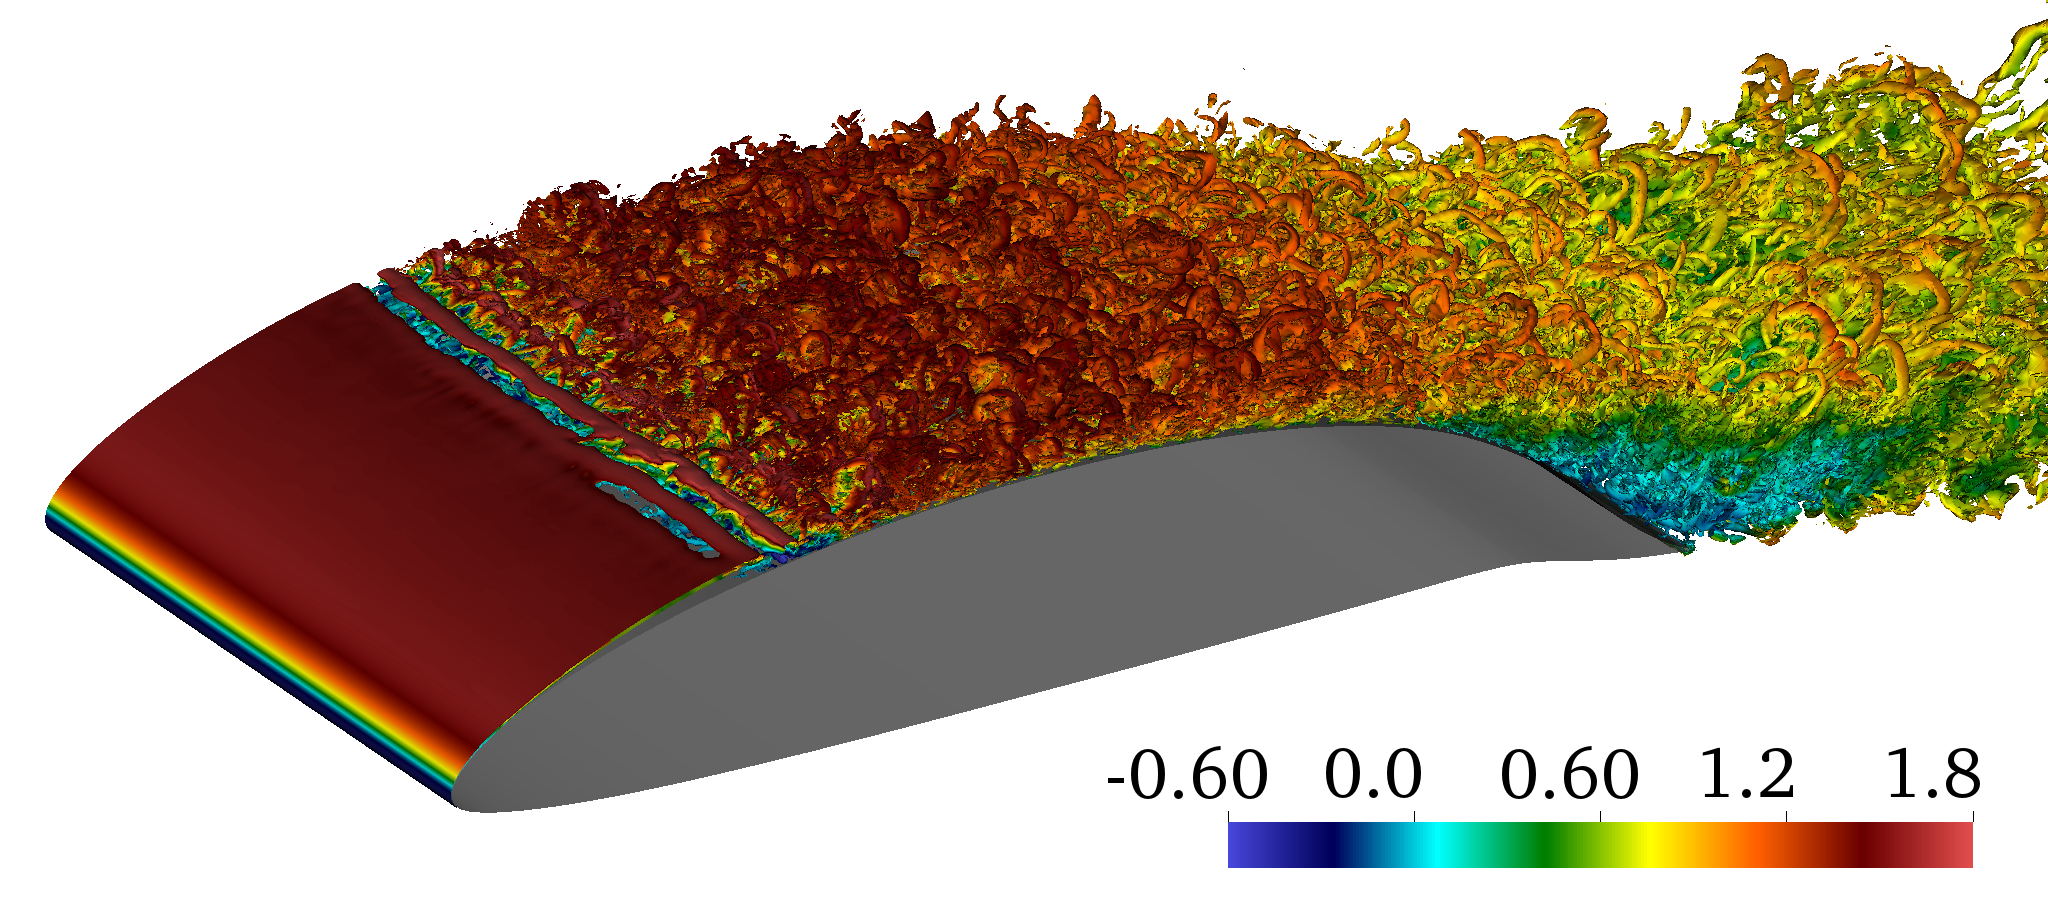
\includegraphics[width=1\textwidth]{pitchup0005.png}
		\label{fig:pitchup_4}
	\end{subfigure}
	\begin{subfigure}[t]{0.49\textwidth}
		\centering
		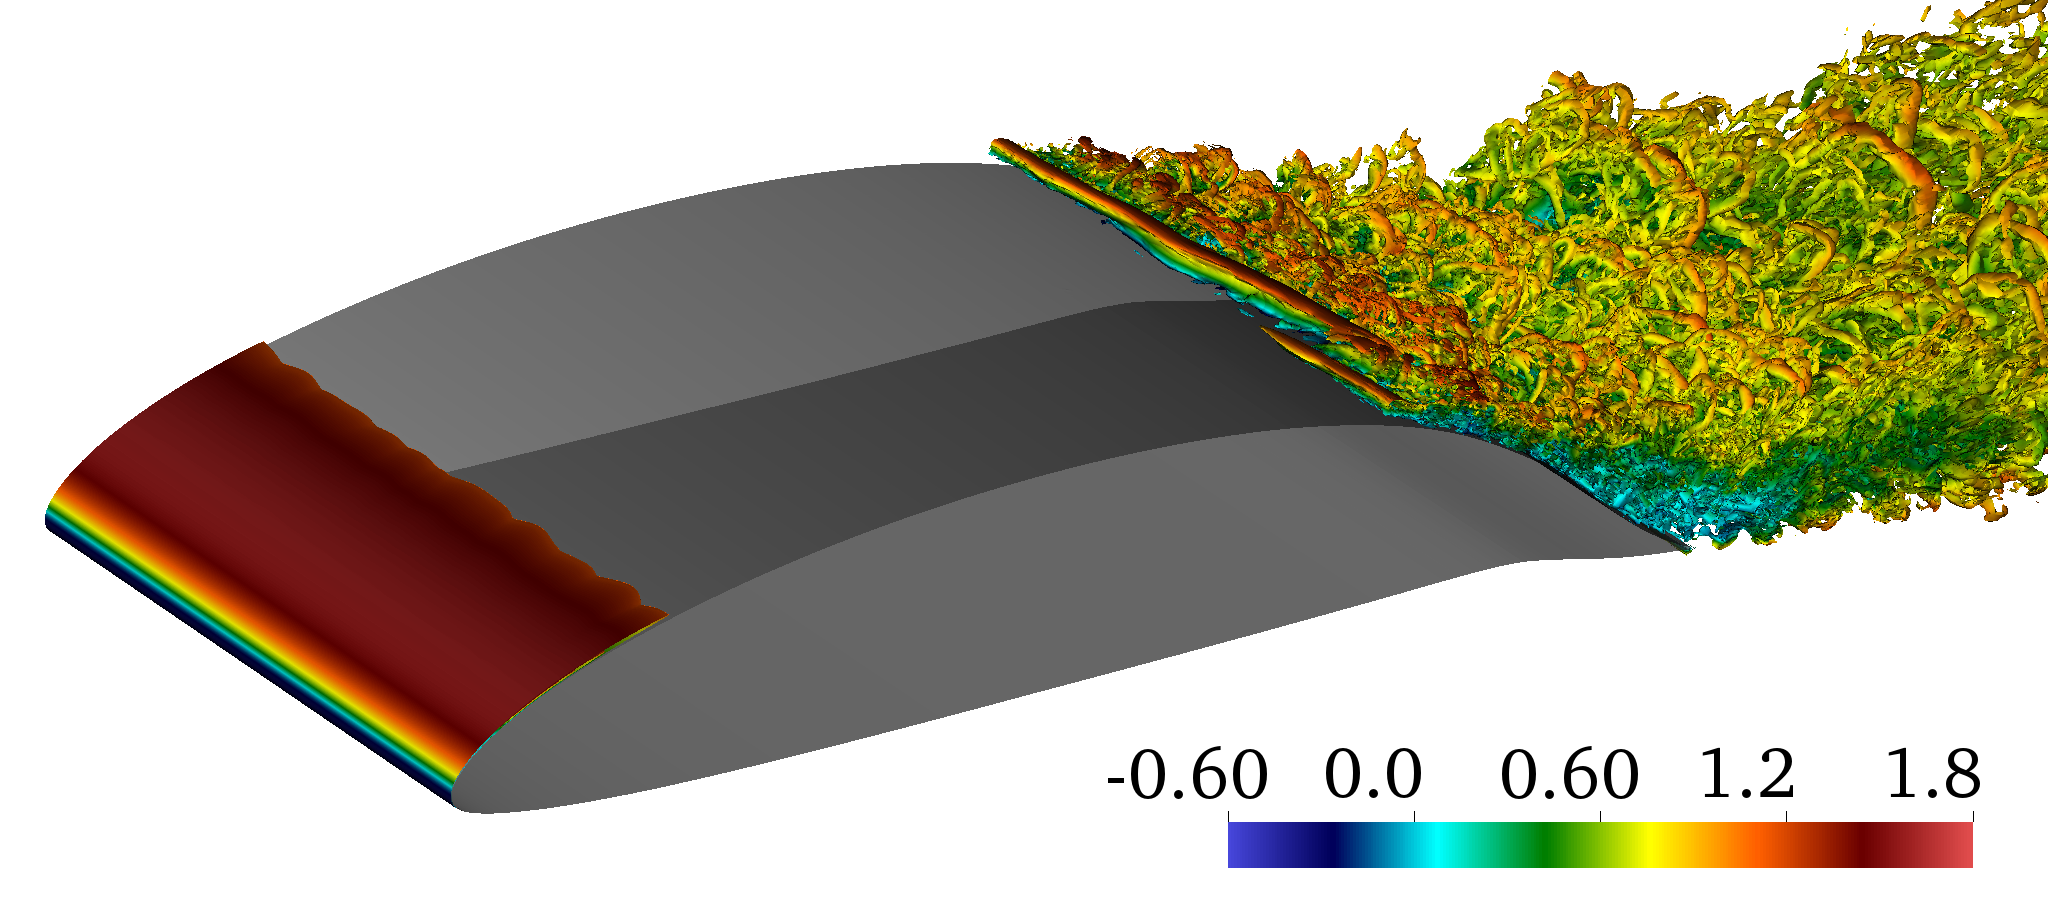
\includegraphics[width=1\textwidth]{relaminar0005.png}
		\label{fig:relaminar_4}
	\end{subfigure}	
	\caption{Visualization of instantaneous $\lambda_{2}$ structures at different phases of the pitch cycle. The figures on the left are during the phase of the pitch cycle when the transition is moving upstream. From top to bottom the time-stamps of the instantaneous snapshots correspond to a normalized flow time of $t/T_{osc}=3.09,\ 3.2,\ 3.3,\ 3.47$. On the right the instantaneous snapshot correspond to the re-laminarization phase as transition moves downstream. The time-stamps from top to bottom on the right correspond to $t/T_{osc}=3.55,\ 3.63,\ 3.82,\ 4.01$}
%	This corresponds to t=19.4015, 20.1655, 20.6975, 21.8295 during the pitchup motion.
%	This corresponds to t=22.3655, 22.8335, 24.0175, 25.2255 during the pitchup motion.	
	\label{fig:transition_la2}
\end{figure}

\begin{figure}
	\centering
	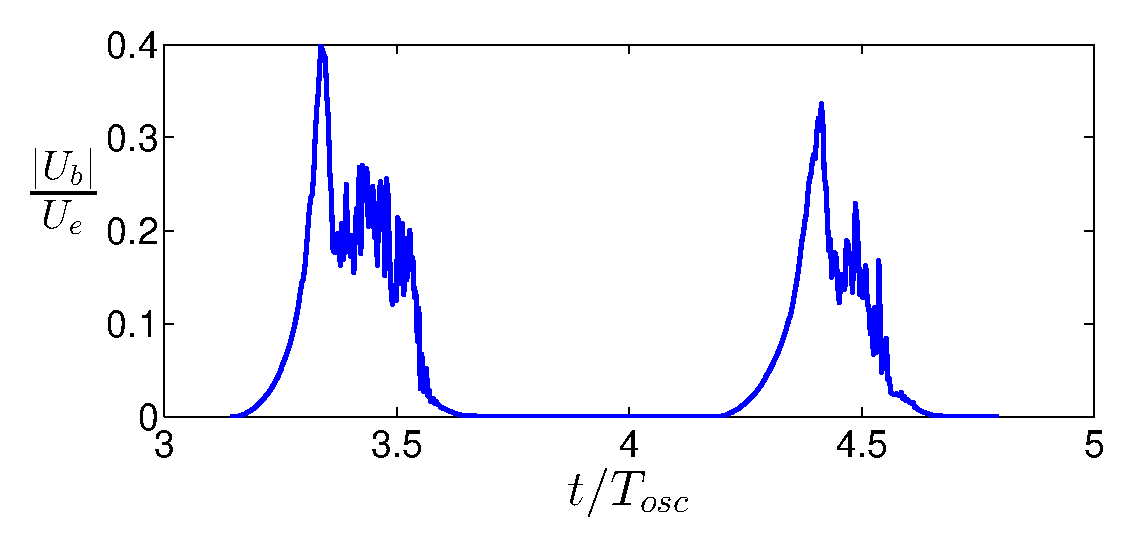
\includegraphics[width=0.6\textwidth]{backflow_ratio}
	\caption{Ratio of maximum reverse flow ($U_{b}$) in the leading edge LSB to the boundary layer edge velocity ($U_{e}$).} 
	\label{fig:backflow_ratio}
\end{figure}

\section{Conclusion}

A relaxation-term filtering procedure is used for wall-resolved LES of flow over a pitching airfoil. The procedure supplements the Navier--Stokes equations with a relaxation term which adds dissipation in the smallest resolved scales of the flow. Validation of the LES procedure is done in a channel flow at $Re_{\tau}=395$ and for a wing section at $Re_{c}=400,000$ and the results show a very good agreement with available DNS data sets.

Flow over an airfoil is simulated using the LES procedure at a chord based Reynolds number of $Re_{c}=100,000$ within an angle of attack range where the aerodynamic forces on the airfoil exhibit sensitive dependence on the angle of attack. This sensitive dependence is captured in the steady simulations at different angles of attack with large changes in transition location within a small variation of $\alpha$.

Pitch oscillations of the airfoil within this $\alpha$ range of sensitive dependence displays a rich variety of unsteady flow phenomena. The flow goes through alternating periods of fully turbulent and laminar flow over the suction side of the airfoil with different governing mechanisms for transition through the oscillating phases. When the flow is mostly laminar over the airfoil surface it separates easily, forming an LSB near the trailing-edge and flow transition  occurs over this separated shear layer. As the angle of attack increases, a leading-edge LSB is formed which first excites strongly spatially growing waves causing transition to move upstream. Eventually the LSB reaches a critical size for transition to occur on the separated shear layer, possibly through an absolute/global instability mechanism. In the pitch-down cycle, the reverse phenomenon occurs where the leading-edge LSB shrinks in size and loses its globally unstable character. Such changing dominance of the trailing-edge and leading-edge laminar separation bubbles creates a continuously changing transition point on the suction side. The upstream and downstream velocities of the transition point movement however are vastly different, with an average upstream velocity being around $V^{tr}_{u}\approx-0.60$ and a much slower downstream velocity of $V^{tr}_{d}\approx0.17$. This asymmetry is yet to be investigated, but may be an important parameter in unsteady turbulence modeling, since this point demarcates the regions of turbulent and laminar flow.

\section{Acknowledgement} 

The computations were performed on resources provided by the Swedish National Infrastructure for Computing (SNIC) at the PDC Center for High Performance Computing at the Royal Institute of Technology (KTH). The work was partially funded by European Research Council under grant agreement 694452-TRANSEP-ERC-2015-AdG. The work was also partially funded by Vinnova through the NFFP project UMTAPS, with grant number 2014-00933. We would like to thank Dr. David Eller and Mikaela Lokatt for providing us with the NLF design and the numerous discussions on different aerodynamic aspects of the project.


%%%%%%%%%%%%%%%%%%%%%%%%%%%%%%%%%%%%%%%%%%%%%%%%%%%%%%%%%%%%%%%%%%%%%%
%\FloatBarrier

%%%%%%%%%%%%%%%%%%%%%%%%%%%%%%%%%%%%%%%%%%%%%%%%%%%%%%%%%%%%%%%%%%%%%%
%\bibliographystyle{tsfp}
%\bibliography{tsfp}
% In this example, BibTeX is used
% For users not familiar with LaTeX, the bibliography can be typed in directly. In this case, comment the two lines above.
%%%%%%%%%%%%%%%%%%%%%%%%%%%%%%%%%%%%%%%%%%%%%%%%%%%%%%%%%%%%%%%%%%%%%%%
%\section*{SAMPLE REFERENCES}
%
%Kwon, O. K., and Pletcher, R. H., 1981, "Prediction of the Incompressible Flow Over a Rearward-Facing Step", Technical Report HTL-26, CFD-4, Iowa State Univ., Ames, IA.
%
%Lee, Y., Korpela, S. A., and Horne, R. N., 1982, "Structure of Multi-Cellular Natural Convection in a Tall Vertical Annulus," Proceedings, 7th International Heat Transfer Conference, U. Grigul et al., ed., Hemisphere Publishing Corp., Washington, D.C., Vol. 2, pp. 221-226.
%
%Sparrow, E. M., 1980a, "Fluid-to-Fluid Conjugate Heat Transfer for a Vertical Pipe - Internal Forced Convection and External Natural Convection", ASME Journal of Heat Transfer, Vol. 102, pp. 402-407.
%
%Sparrow, E. M., 1980b, "Forced-Convection Heat Transfer in a Duct Having Spanwise-Periodic Rectangular Protuberances", Numerical Heat Transfer, Vol. 3, pp. 149- 167.
%
%Tung, C. Y., 1982, Evaporative Heat Transfer in the Contact Line of a Mixture, Ph.D. Thesis, Rensselaer Polytechnic Institute, Troy, NY.

%%%%%%%%%%%%%%%%%%%%%%%%%%%%%%%%%%%%%%%%%%%%%%%%%%%%%%%%%%%%%%%%%%%%%%


%\end{document}
